\documentclass{tfg_domingo}
% \documentclass[numeros]{tfg_domingo}
\usepackage{graphicx} % Required for inserting images
%\usepackage{algorithm}
\usepackage{algpseudocode}
\usepackage{amsmath}
\usepackage{amssymb}
\usepackage{stackengine}
\usepackage{comment}
\usepackage{tcolorbox}
\usepackage{listings}
\usepackage{scalerel}
\usepackage{xcolor}
\usepackage{karnaugh-map}
\usepackage{hyperref}
\definecolor{fuchsia}{RGB}{255, 0, 255}
\lstdefinestyle{goneStyle}{
  language=Java, % Set the language to Python for syntax highlighting
  basicstyle=\ttfamily\small, % Set the font family and size
  keywordstyle=\color{fuchsia}, % Set the color for keywords
  commentstyle=\color{green!60!black}, % Set the color for comments
  stringstyle=\color{red}, % Set the color for strings
  showstringspaces=false, % Don't show spaces in strings as underscores
  numbers=left, % Show line numbers on the left
  numberstyle=\footnotesize\ttfamily\color{gray}, % Set the style for line numbers
  frame=single, % Add a frame around the code
  rulecolor=\color{lightgray}, % Set the color for the frame
  breaklines=true, % Enable line breaks
  breakatwhitespace=true, % Break lines at whitespace
  tabsize=4 % Set the tab size
}
\lstdefinestyle{pythonStyle}{
  language=Python, % Set the language to Python for syntax highlighting
  basicstyle=\ttfamily\small, % Set the font family and size
  keywordstyle=\color{fuchsia}, % Set the color for keywords
  commentstyle=\color{green!60!black}, % Set the color for comments
  stringstyle=\color{red}, % Set the color for strings
  showstringspaces=false, % Don't show spaces in strings as underscores
  numbers=left, % Show line numbers on the left
  numberstyle=\footnotesize\ttfamily\color{gray}, % Set the style for line numbers
  frame=single, % Add a frame around the code
  rulecolor=\color{lightgray}, % Set the color for the frame
  breaklines=true, % Enable line breaks
  breakatwhitespace=true, % Break lines at whitespace
  tabsize=4 % Set the tab size
}
\newcommand{\comentario}[1]{\textcolor{red}{#1}}
\autor{Pedro Castro Cutillas}
\titulo{Construcción de un compilador para el lenguaje BeGone}
% Título corto para los encabezamientos de pagina:
\corto{} % En blanco si no es necesario recortarlo.
\ingles{Construction of a Compiler for the BeGone Language}
\fecha{Septiembre - 2024}
% La normativa prescribe «cuatro o cinco palabras clave, en
% español y en inglés, para su indexación en el repositorio
% de TFG».
\palabras{Compilador, Lexer, Parser, Python3, Algoritmo de Compresión}%
  {Compiler, Lexer, Parser, Python3, Compression algorithm}

\usepackage{amsthm} % Esto solo es relleno.
\usepackage{lipsum}
\usepackage{graphicx}
\usepackage{caption}
\usepackage{subcaption}
\usepackage{comment} 


\newtheorem{Def}{Definition}
%\newtheorem{Proof}{Proof}
\newtheorem{Th}{Theorem}
\newtheorem{Algorithm}{Algorithm}
\newtheorem{Lemma}{Lemma}
\newtheorem{Prop}{Proposition}
\newtheorem{Corollary}{Corollary}
\providecommand{\abs}[1]{\lvert#1\rvert}
\providecommand{\norm}[1]{\lVert#1\rVert}
\renewcommand{\exp}[1]{e^{#1}}

\begin{document}
%ejemplo: \href{https://www.youtube.com/watch?v=sPiWg5jSoZI}{Python 3 Metaprogramming}
% Si alguna palabra se divide entre dos líneas en un punto
% indebido, podemos indicar aquí los puntos de corte
% aceptables (si los hay), p. ej,
% \hyphenation{ba-rro-co, frío, cria-do, su-per-ra-tón}
\hyphenation{Dijkstra new-speak}
\SetKwComment{Comment}{/* }{ */}
\portada        
\frontmatter
\gracias{\input{agradecimientos.txt}}
\resumen{%El problema del conteo de personas en imágenes resulta de vital importancia en tareas de seguridad pública y control de masas en eventos multitudinarios. La tecnología actual utiliza diferentes metodologías automáticas para diseñar y entrenar distintos modelos de redes neuronales. Por otro lado, existen métodos de conteo manual donde el objetivo es obtener una estimación con el menor número de muestras posibles. Los métodos manuales se basan en una ciencia matemática llamada estereología, pero su aplicación ha quedado en segundo plano por la ingente cantidad de datos que ahora permiten entrenar redes neuronales con bastante precisión. En este trabajo se plantea hacer una revisión sistemática de la literatura de los dos campos. Se tratará de combinar los métodos de estereología con las redes neuronales para comprobar si la estereología ha quedado suplantada o sus fundamentos pueden lograr avances en este campo. 



%La estereología es la ciencia del muestreo geométrico y permite estimar cantidades utilizando fórmulas que suelen incluir esperanzas. En este trabajo se han intentado mejorar los estimadores usados en estereología aproximando dichas esperanzas mediante el uso de integración QMC con $N$ puntos óptimos que minimizan el \textit{worst-case-error} para el \textit{reproducing kernel Hilber space} $H_{mix}^1$. Este proceso debería dar estimadores con poca varianza, mejorando la calidad de la cantidad estimada.\\
%Para comprobar el funcionamiento de este proceso se han seleccionado tres \textit{test systems} conocidos, el \textit{test system de quadrats}, el \textit{Buffon test system} y el \textit{Buffon-Steinhaus test system}, y se ha implementado en un código python para cada uno.\\
%Los resultados calculados por ordenador apuntan a que este proceso puede que funcione mejor o peor dependiendo de la isotropía, anisotropía o simetría que tiene el objeto de cuya cantidad se quiere estimar. %También es posible que cambiando un cierto parámetro $\gamma$ (ver \cite{Hinrichs.pdf}) se obtengan mejores resultados al usar ese proceso, pero aún así permite obtener estimadores precisos con bajo error.\\

%----------------------------------------------------------------------------------
%Stereology is the science of geometric sampling and it allows to estimate quantities using formulas that usually include expectations. Artificial Intelligence is a discipline in computer science that encompasses several different processes concerned with making machines smart. In this work we combined both Stereology and AI in order to test a new method for Crowd Counting, an AI field that revolves around the estimation of the number of individuals in images or videos. Our method's approach considers a modified test system of quadrats whose quadrats are only located at the points contained in an Optimal Point Set that minimizes the worst case error for Quasi-Monte Carlo Integration. By superimposing the system to an image and cropping that image by the quadrats, we can then use an AI model to count individuals on each crop, subsequently using Equations \ref{Conteo_usada} and \ref{QMC} to estimate the total count value of individuals in the original image. The chosen AI model to try our method was CLIP-EBC, as it is a public model and one of the best performing models in crowd-counting. The computed results for the validation metrics MAE and RMSE suggest that there is a lot or research to be made regarding our method, however, the best variant tested for our method is not far from performing in a similar level to that of the state-of-the-art methods in Crowd Counting. What's more, the computing times obtained for that variant are much lower than those obtained by one of the best performing methods, CLIP-EBC.\\

La estereología es la ciencia del muestreo geométrico y permite estimar cantidades utilizando fórmulas que suelen incluir esperanzas. La inteligencia artificial es una disciplina en ciencias de computación que engloba varios procesos relacionados con crear máquinas inteligentes. En este trabajo se han combinado la estereología y la IA de cara a probar un nuevo método de conteo de multitudes (Crowd Counting), el área centrada en estimar el número de individuos en imágenes o vídeos. El planteamiento de nuestro método considera un \textit{test system} (sistema de testeo) de quadrats modificado cuyos quadrats sólo se posicionan en los puntos contenidos en un conjunto de puntos óptimo que minimiza el \textit{worst case error} (error en el peor caso) para la integración Quasi-Monte Carlo. Superponiendo este \textit{test system} a una imagen y recortándola en los quadrats podemos usar el modelo de IA para contar individuos en cada recorte y, posteriormente, usar las Ecuaciones \ref{Conteo_usada} y \ref{QMC} para estimar la cantidad total de individuos en la imagen original. El modelo de IA escogido para probar nuestro método ha sido CLIP-EBC, dado que es un modelo público y uno de los modelos con mejores resultados en conteo de multitudes. Los resultados computados para las métricas de validación MAE (error absoluto medio) y RMSE (error cuadrático medio) muestran resultados esperanzadores respecto a nuestro método. %%DomingoMaster: Esto, aunque esta bien, me parece un poco repetitivo.
%Aunque, la mejor variante probada de nuestro método no está lejos de rendir a un nivel similar al de los métodos más recientes de conteo de multitudes. 
Lo que es más, los tiempos de cómputo obtenidos para dicha variante son mucho más bajos que los obtenidos por uno de los modelos que mejores resultados obtiene, CLIP-EBC.\\





}{%Stereology is the science of geometric sampling and it allows to estimate quantities using formulas that usually include expectations. In this work we tried to improve stereology estimators by approximating the expectations using QMC integration with $N$ optimal points that minimize the worst case error in the reproducing kernel Hilbert space $H_{mix}^1$. This process should provide estimators with low variances, improving the quality of the estimated quantity.\\
%In order to test this process we selected three known test systems, namely the test system of quadrats, the Buffon test system and the Buffon-Steinhaus test system, and implemented it in python code for each one of them.\\
%The computed results led us to think that this process might perform differently depending on the isotropy, anisotropy or symmetry that the object whose quantity we estimate has. %Also, it's possible that changing a certain parameter $\gamma$ (see \cite{Hinrichs.pdf}) may provide better results when using that process, but it still gives low error accurate estimators.\\
(tiempo presente, primera persona del plural, hablando de lo que se ha conseguido en el TFG)
Stereology is the science of geometric sampling and it allows to estimate quantities using formulas that usually include expectations. Artificial Intelligence is a discipline in computer science that encompasses several different processes concerned with making machines smart. In this work we combined both Stereology and AI in order to test a new method for Crowd Counting, a field that revolves around the estimation of the number of individuals in images or videos. Our method's approach considers a modified test system of quadrats whose quadrats are only located at the points contained in an Optimal Point Set that minimizes the worst case error for Quasi-Monte Carlo Integration. By superimposing the system to an image and cropping that image by the quadrats, we can then use an AI model to count individuals on each crop, subsequently using Equations \ref{Conteo_usada} and \ref{QMC} to estimate the total count value of individuals in the original image. The chosen AI model to test our method was CLIP-EBC, as it is a public model and one of the best performing models in crowd-counting. The computed results for the validation metrics MAE and RMSE shows promising results.
%%DomingoMaster: Creo que da un poco repetitivo.
%however, the best variant tested for our method is not far from performing in a similar level to that of the state-of-the-art methods in Crowd Counting. 
An additional benefit is  the computing times obtained for that variant are significantly lower than those obtained by the most optimised performing methods, CLIP-EBC.\\

}
\tableofcontents

\mainmatter
% PREGUNTAR COMO ARREGLAR MAYUSCULAS
\chapter{Introduction}\label{cap:Intro}
\section{Motivación}
Los compiladores son un pilar fundamental en la tecnología contemporánea. Estos han conseguido facilitar la programación construyendo capas de abstracción entre la máquina y el programador. Antes se programaba directamente en código ensamblador que después se traducía al código máquina para generar un ejecutable. A día de hoy, lo más común es programar en lenguajes de alto nivel como \textit{Python} o \textit{JavaScript}, donde hay miles de librerías y herramientas que ofrecen múltiples funcionalidades para que facilitar el desarrollo de software de cualquier tipo. \\
Se debe hacer una clara distinción entre compilador e interprete, el compilador traduce todo el código fuente del lenguaje original a código máquina, lo cual evidentemente le hace en la mayoría de casos más rápido. Sin embargo, el interprete convierte cada línea, una a una a código máquina teniendo en cuenta los resultados de líneas anteriores con técnicas como el conteo de referencias, garbage collection, etc... \\
En la primera parte de este trabajo hablaremos del desarrollo de un compilador. He escogido escribir un compilador porque siempre me ha interesado conocer lo que realmente ocurre en la computadora cuando tras escribir tu programa genera un ejecutable. Y porque creo que conocer detalles de programación de bajo nivel son de ayuda en el día a día de un programador. Además, conocer todas las etapas por las que pasa el código fuente hasta convertirse en código máquina te da una perspectiva global sobre la naturaleza de un lenguaje de programación de alto nivel.\\
En cuanto a la segunda parte del trabajo, los algoritmos de compresión siempre habían llamado mi atención. Sin embargo, nunca me había tomado el tiempo para analizar ninguno de ellos. Con este trabajo he tenido la oportunidad de profundizar en conceptos como los registros de desplazamiento, o las formulas lógicas que antes desconocía.\\
En conclusión, la motivación principal de este trabajo era conocer en mayor profundidad los compiladores y los algoritmos de compresión, que en cierta manera se entremezcla con algunos algoritmos de cifrado.

\section{Objetivos}
El primer objetivo de este proyecto era crear un compilador funcional del lenguaje BeGone, siguiendo las lecciones del curso de David Beazley. El curso contiene lecciones básicas para guiarte y después escribir tu propia implementación, algunos tests, y un compilador medio implementado para que compruebes si la salida de tu compilador coincide con la de este. Este compilador de ayuda deja de ser útil a partir de la implementación básica del módulo de generación de código llvm. A partir de ese punto, aunque existen tests, está poco guiada y presenta grandes retos. Esta parte del desarrollo abarca el desarrollo de los booleanos, las comparaciones, el control del flujo (sentencias \textit{if}, \textit{ifelse} y \textit{while}) y las funciones, que son las secciones que más tiempo y más complejas son de implementar. \\\\
Después del desarrollo completo del compilador, mi tutor me ofreció un artículo \cite{limniotis2007nonlinear} donde había un algoritmo que daba como generar eficientemente  una secuencia binaria. El algoritmo presentaba limitaciones y el problema planteado fue si esa forma era la más eficiente posible para la compresión de ficheros, lo que derivo a desarrollar un formato de archivo especial para este algoritmo. Y con este formato, implemente en el compilador original dos funciones nativas para codificar y decodificar un archivo. Evidentemente, esto provoco cambios en todas las etapas del compilador. Al hacer esto el compilador original paso de llamarse BeGone a GoneFSR. \\\\
El último de los objetivos fue desarrollar una memoria técnica donde todo fuera claro para el lector a la vez que didáctico. Para ello, tome como inspiración la estructura de la sección del desarrollo del compilador, el documento \href{https://repositorio.unican.es/xmlui/handle/10902/30046}{intérprete Lox} ofrecido por mi tutor. Para la segunda parte del proyecto, los conceptos se explican desde los más sencillos hasta los más complejos, para que el lector no reciba estos últimos de golpe.

\section{Desarrollo software}
Para el desarrollo del compilador el modelo de desarrollo software utilizado ha sido el modelo incremental iterativo, tal y como se recomienda en el curso de BeGone. Este consiste en dividir el proyecto en etapas, y para cada etapa aplicar las distintas fases de desarrollo para producir un software sin errores. Estas etapas se desarrollan secuencialmente, aplicando pequeños incrementos en la complejidad del proyecto después de haberse asegurado que la etapa anterior estaba bien desarrollada. En cada incremento el objetivo es añadir o extender una funcionalidad en el proyecto global, a cada incremento se lo podría asociar con un hito si se conoce el \textit{framework} \textit{SCRUM}. \\\\
Al desarrollar el proyecto de esta manera puedes aplicar tests en cada etapa, haciendo así que el feedback dado por los tests tanto unitarios (caja negra) como de sistema (caja blanca) sea más fácil de entender y aplicar las correcciones necesarias implique menos trabajo. \\\\
En la práctica he creado un repositorio git en local y he trabajado sobre dos ramas una \textit{dev} y otra \textit{prod}. Haciendo commit en \textit{dev} por cada pequeño avance, y haciendo merge en \textit{prod} cada vez que completaba una etapa del desarrollo. Podéis consultar el código en el ~\href{https://github.com/domingoUnican/TFGPedroCastro/tree/main/code}{repositorio}. Debo mencionar que  no está el historial de logs pertinente. Ya que el compilador fue desarrollado en mayo, y no subí el repositorio original a mi github. \\\\
Por último, respecto al desarrollo de \textit{scripts} y otros experimentos relacionados con la segunda parte del proyecto, no he seguido ningún estándar. Ya que solían ser pruebas separadas y no un proyecto global, que necesitase de planificación y estructura.

\section{Herramientas y apoyos} 
Para el desarrollo del compilador se han usado la librería SLY (Sly Lex Yacc), que tiene como antecesores dos herramientas muy conocidas llamadas lex y yacc (Yet Another Compiler Compiler). Esta librería me ha permitido no tener que implementar el autómata finito del \textit{Lexer}. Además de ahorrarnos el desarrollo de la estructura del \textit{Parser} permitiendonos focalizarnos en la definición de la gramática libre de contexto.


\chapter{Compilador GoneFSR}\label{cap:Teoria}

Hoy en día es sencillo para cualquier persona con la suficiente motivación aprender a programar. De hecho, para programar en \textit{JavaScript} (ECMAScript) utilizando un entorno de ejecución como \textit{NodeJS} sobre un framework como \textit{React}, ni siquiera necesitas conocimientos sobre \textit{hardware}, ni saber como se gestiona la memoria, ni hasta cierto punto la naturaleza de un "puntero". Sin embargo, podríamos decir que estarías "programando". Creo que cada vez es más accesible y tenemos más herramientas para poder plasmar nuestras ideas a través de la propia programación, y a la vez tanta abstracción nos aleja de la cantidad de pasos que hay detrás de cada línea de código.\\\\
La primera vez que intente programar tenía trece años, e intente aprender \textit{Java} mediante unos tutoriales de \textit{Youtube}. En uno de los primeros vídeos, explicaba como se compila el código y las fases que atraviesa hasta convertirse en código máquina. Allí, lo explicaban de manera muy sencilla, primero tienes el código fuente, ese código se transforma en \textit{bytecode} (o código intermedio), y ese \textit{bytecode} pasa por una máquina virtual (JVM, Java Virtual Machine) para convertirse en código máquina. Resulta que el proceso de compilación me llamó la atención, y es por esto que he escrito mi propio ``mini''  lenguaje, al que he llamado GoneFSR, siguiendo las instrucciones y la estructura que propone David Beazley en su curso. (estos dos parrafos tal vez haya que pasarlos a la introduccion)\\\\
El compilador está basado en el curso de David Beazley, en el que explica como desarrollado un compilador llamado \textit{BeGone}, sin embargo debido a algunas extensiones de este compilador que se han realizado además de la completa implementación de las funcionalidadas requeridas por el curso, he decidido llamarlo GoneFSR. \\\\
En las siguientes subsecciones analizaremos cada parte que componen este compilador frontend. Cuando compilas código en GoneFSR, el compilador pasa por varias etapas: análisis sintáctico, análisis semántico, análisis de errores, generación de código intermedio y generación de código llvm (Low Level Virtual Machine). Ese código llvm será traducido a un ejecutable por CLANG, como último paso. A continuación veremos que significa todo esto, además de algunos detalles sobre la implementación de cada etapa.
\newpage
\section{Análisis léxico}
En un idioma cualquiera,  el léxico se entiende como el conjunto de palabras y expresiones que pertenecen a esa lengua. Al módulo del compilador, encargado del análisis léxico o tokenizado se le suele llamar \textit{Lexer}. Y su función, es por consiguiente asegurarse de que todas las palabras del archivo de entrada, pertenecen al lenguaje de programación. \\\\
Para poder llevar a cabo este proceso, el \textit{Lexer} divide la cadena de caracteres de entrada (contenido del archivo ``.g``)en \textit{tokens}. Para encontrar cada token recorre la cadena implementando un autómata finito que transiciona de estado en función del carácter que está recorriendo pasa de un estado a otro y acaba devolviendo los tipos de tokens que hemos definido en la clase como expresiones regulares. El orden en el que se definen los tokens tiene importancia, definir un token antes que otro en los que los dos comparten el comienzo del patrón, significa que se le dará prioridad al definido previamente, es por esto que todos los tokens del lenguaje se definen antes que los identificadores, ya que la REGEX de los identificadores engloba a palabras clave, como ``bool`` o ``char``. (grafismo lexer como en tfg Eduardo)
\\\\
Por \textit{token} se entienden todo tipo de palabra tanto clave como identificador, así como delimitadores como los paréntesis o el punto y coma. Aunque la función principal del \textit{Lexer} es generar tokens, también se encarga de ignorar algunos caracteres que no necesitamos que se traten como \textit{tokens} para que estos no pasen a la segunda fase, que sería el \textit{parsing} o análisis semántico, un buen ejemplo de esto son los caracteres de salto de línea, o los comentarios.\\\\
En GoneFSR, hay cuatro tipos distintos de datos. 
\begin{itemize}
    \item{Números enteros (int) de 32bits}
    \item{números decimales (float), este tipo de dato normalmente se asocia a números de coma flotante 32 bits, pero en este lenguaje en la fase final de compilación se mapean a double (64 bits) en las instrucciones llvm}
    \item{carácter (char)  es simplemente un único carácter estando permitidos cualquier letra o número, además de caracteres especiales como \textbackslash, \textbackslash n, \textbackslash ", \textbackslash xhh (siendo hh cualquier valor hexadecimal lo que permite representar cualquier carácter ASCII).}
    \item{cadenas de carácteres (strings) se especifican con la sintaxis ``texto`` y es importante decir que no se puede iterar sobre ellas. }\\
\end{itemize}
Todos las sentencias en GoneFSR, deben acabar en ";", como por ejemplo en lenguajes como C, o Java. En este lenguaje existen variables mutables e inmutables, para las inmutables o constantes no es necesario especificar un tipo de dato ya que se infiere del propio dato. La sintaxis para constantes sería
\begin{lstlisting}[style=goneStyle]
const ID = value;
\end{lstlisting}
En el caso de las variables mutables si se requiere que el usuario especifique un tipo de dato en concreto de los cuatro disponibles. La sintaxis sería
\begin{lstlisting}[style=goneStyle]
var ID datatype = value;
\end{lstlisting}
Las operaciones binarias disponibles en el compilador tanto para enteros como para decimales son: suma, resta, multiplicación y división. Siguiendo el estándar cada una de ellos se asocia con los símbolos +, -, *, /, respectivamente.\\\\
El compilador cuenta con las siguientes operaciones condicionales para después con las sentencias condicionales (``conditional statements``) poder  bifurcar el código, menor que ($<$), mayor que ($>$), menor o igual que ($\leq$), mayor o igual que ($\geq$), igual que (==) y no igual que (!=), todas estos operadores funcionan tanto para int como para float, pero no se pueden comparar entre tipos, siempre tienen que ser comparaciones entre el mismo tipo, ya que en este lenguaje no están implementados los \textit{castings} a otros tipos. Las comparaciones entre booleanos son las siguientes: igual que (==), no igual que (!=), ``y`` ($\And\And$) y ``o`` ($||$).\\\\
El símbolo + y -, también actúan como operadores unarios para int y float, para especificar cuando un número es positivo o negativo. Para lo booleanos existe el operador unario !, el cual sirve para negar el valor de la variables booleana. \\\\
\newpage
\noindent La primera sentencia condicional es el clásico "if", el cual cuenta con una sintaxis ampliamente extendida entre otros lenguajes.

\begin{lstlisting}[style=goneStyle]
if (condition) {
    statements
}
\end{lstlisting}

\noindent Para escribir un "if else".

\begin{lstlisting}[style=goneStyle]
if (condition) {
    statements
}
else {
    statements
}
\end{lstlisting}

\noindent En caso de querer escribir un bucle, GoneFSR, tan solo cuenta con el bucle ``while`` por simplicidad, que se escribiría con la sintaxis.

\begin{lstlisting}[style=goneStyle]
while (condition) {
    statements
}
\end{lstlisting}

\noindent Ya solo nos queda por ver como se declaran las funciones. En GoneFSR las funciones se escriben tal que así.
\begin{lstlisting}[style=goneStyle]
func function_name (*arguments) return_datatype {
    statements
}
\end{lstlisting}
Las funciones en GoneFSR siempre tienen que retornar un tipo de dato, ya que no existe el tipo de dato void como en C. Todos los flujos de cualquier función escrita deben retornar algo, si no el \textit{checker} lo evaluará como un error, el mecanismo para lograr esto es bastante interesante, en la sección análisis de errores, veremos como está implementado en detalle. Todo código que este escrito fuera de una función, se considera \textit{global}, aún no lo había mencionado pero en GoneFSR sí esta implementado un \textit{scope} propio para cada función así que cada una tiene su propio espacio para las variables. A nivel interno, por como está construido el compilador valore que la mejor opción era agrupar todo el código escrito fuera de una función y escribirlo en una función llamada ``\textit{premain}``, para luego en la función \textit{main} escribir como primera instrucción la llamada a esta función \textit{premain}.



En GoneFSR, hay dos funciones ``built-in``, es decir las puedes llamar sin necesidad de importar nada, ``print`` y ``filetonlfsr``. Desgraciadamente GoneFSR, no cuenta con implementaciones de gestor de módulos, ni \textit{garbage collection}, ni control de importaciones circular, ya que al fin y al cabo, no deja de ser un compilador con un propósito educativo.\\\\
\newpage
\noindent ¿Pero, cómo se distingue cada token, cómo se distingue un ``if`` de un  ``print``?, pues bien, en este caso haremos uso de la librería o mejor dicho, módulo de Python llamado SLY (Sly Lex Yacc). Esta librería que a su vez de dos herramientas muy conocidas llamadas lex y yacc (Yet Another Compiler Compiler), nos facilita el desarrollo de tanto lexers como parsers para el desarrollo de compiladores. Concretamente, nos facilita dos clases  \textit{Lexer} y \textit{Parser}, que nos harán más amigable el proceso de parsing y tokenizado del código fuente de nuestro lenguaje. \\\\
Pero, para abstraernos del código, explicaré lo esencial de la implementación del \textit{Lexer}. La clave está en las expresiones regulares, más conocidas como REGEX, estas nos permitirán buscar patrones y encontrar los tokens que queremos.\\\\
Dominar las expresiones regulares es complejo, hay muchas reglas que debes conoces, muchas caracteres que dependiendo del contexto significan una cosa u otra: grupos de captura, contenedores, ``lookahead`` con condiciones, caracteres comodín, etc... \\\\
Describir el funcionamiento de estos, me llevaría probablemente otras diez páginas así que consideraré que con decir que es a través de estas expresiones regulares como capturamos los \textit{tokens}, es suficiente. Para que no queden sin explicar, pondré un ejemplo, cómo distinguimos los enteros.
\begin{lstlisting}[style=pythonStyle]
INTEGER = r'0x[a-f0-9]+|0o[0-7]+|0b[10]+|d+'
\end{lstlisting}
\noindent Para aquellos entendidos en expresiones regulares, sabrán que hay un detalle que me he saltado sobre los enteros. Y es que un entero puede escribirse sobre diferentes bases, se puede escribir, en base diez, en base dos (binario), en base ocho (octal) y en base dieciséis (hexadecimal). En la expresión regular se puede distinguir que se define como un entero la cadena '0x' seguida de al menos un (símbolo +) carácter 'a', 'b', 'c', 'd', 'e' y 'f' o de un dígito del cero hasta el nueve. Con esta configuración no se aceptaran como caracteres hexadecimales aquellos escritos con letras mayúscula, esto es una decisión arbitraria, ya que sería fácil admitirlos. Con el carácter '$|$' especificamos un 'or' en la expresión es decir que también pueden admitirse escritos en octal (comenzando con '0o' y seguidos de al menos un dígito del cero al siete), escritos en binario (comenzando con '0b' y seguidos de al menos un dígito del cero al uno), o escritos en decimal que es lo que quiere decir la subcadena 'd+', es decir al menos un dígito del cero al nueve. \\\\
Para cada uno de los \textit{tokens} del lenguaje hay una expresión regular que lo describe, para consultar todas las expresiones regulares, tenéis el código original en \href{https://github.com/domingoUnican/TFGPedroCastro/blob/main/code/compilerGoneFSR/gone/tokenizer.py}{tokenizer.pyº}.



\newpage
\section{Análisis semántico}
Un \textit{token} no es nada por si solo, lo que lo define es como se relaciona con los otros \textit{tokens}. La definición de las relaciones entre tokens se le llama gramática. Y es en el \textit{Parser} donde hay que establecer las reglas de esta gramática. Estas reglas serán las que le den forma al AST (Abstract Syntax Tree) de cada programa de nuestro lenguaje, más tarde explicaremos qué es y pondremos un ejemplo de un AST.\\\\
Nos basaremos en la notación BNF (Backus Naur Formalism) para definir nuestra gramática libre de contexto, esta es la parte más importante, pues si todas las reglas están bien escritas pasarlo al \textit{Parser} será sencillo. Sin embargo, en este paso es fácil quedarse atascado pues hay que ser meticuloso con cada regla que escribes, ya que si no defines una buena estructura para el AST, los siguientes pasos pueden hacerse sumamente tediosos. \\\\
En el apéndice podéis consultar las reglas de la gramática. No entraré en detalles de la implementación porque no me parece relevante, pues si entiendes la gramática, entender la estructura de la clase \textit{Parser} es sencillo. Debo mencionar que esta sección del compilador realmente son dos clases en el proyecto, evidentemente, una de ellas es la clase \textit{Parser} que hereda directamente de la clase \textit{Parser} de SLY, pero la otra clase, es la clase encargada de definir las clases de cada nodo del AST. Hay muchas maneras de definir estos nodos, pero lo importante es que quede muy claro que nodos pueden estar asociados a su vez con otros nodos. Por ejemplo el nodo "ConstDeclaration" tiene como atributos un nombre de tipo "string" y un valor de tipo "Expression", o el nodo "BinOp" (Binary Operation) que tiene como atributos el tipo de operación, el operando izquierdo y el operando derecho.\\\\ 
Todo esto se entiende mucho mejor con un ejemplo de un AST de un programa en GoneFSR. Es un ejemplo muy sencillo, pero la idea creo que puede quedar clara con esto. Este sería el código fuente.

\begin{lstlisting}[style=goneStyle]
func main () int {
    var b int = 1;
    if 1 < 3 {
        b = 7;
        print b;
    }
    return 0;
}
\end{lstlisting}


\newpage Y este el AST asociado generado por el compilador en base a ese código.
\begin{figure}[h]
    \centering
    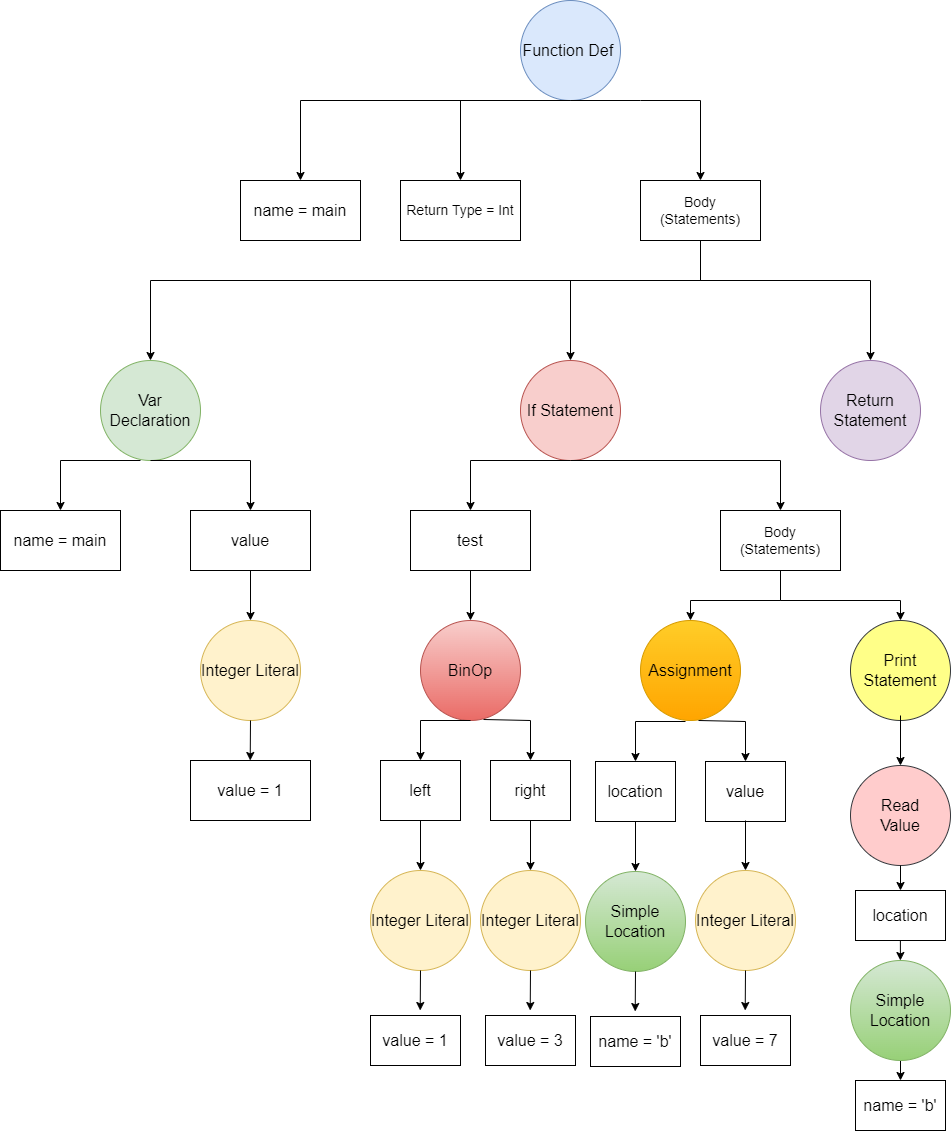
\includegraphics[width=0.9\textwidth,keepaspectratio]{img/asttree_latexexample.png} 
    \parbox{\linewidth}{\centering Ejemplo AST}
    \label{fig:mi_imagen}
\end{figure}

\newpage
(queda hablar sobre la precedencia)El AST es importante porque en los siguientes pasos lo que haremos será recorrer recursivamente este árbol para analizar errores y finalmente, generar el código intermedio. El código del \textit{Parser} se encuentra en \href{https://github.com/domingoUnican/TFGPedroCastro/blob/main/code/compilerGoneFSR/gone/parser.py}{parser.py}.
\section{Análisis de errores}
Analizar errores es un proceso complicado de programar, hay muchas cosas que pueden fallar en tiempo de ejecución y un buen compilador debe dar feedback al programador de las cosas que debe corregir para que su programa, al menos compile. Porque eso es en esencia, a lo que se dedica esta sección, a asegurarse de que todo el código fuente tiene sentido semántico, y si no lo tiene, corta el flujo del programa y no lo deja pasar a la generación de código intermedio.  \\\\
En esta fase, el compilador GoneFSR, se asegura de que todos los identificadores estén definidos antes de que se les haga referencia. Avisa de todos aquellos errores de tipado como por ejemplo asignar un valor de tipo char a una variable de tipo int. Se asegura de que las comparaciones se hacen entre valores o variables del mismo tipo de dato. Notifica si se intenta cambiar el valor de una variable cuando se trata de una constante. Revisa que no llames a una variable con el nombre de un tipo de dato, ya que estas son palabras reservadas. Todo esto, entre muchos más "\textit{checks}" que se pueden consultar en el fichero \href{https://github.com/domingoUnican/TFGPedroCastro/blob/main/code/compilerGoneFSR/gone/checker.py}{checker.py}.
\\\\
En cuanto a como se recorre el árbol, es sencillo, por cada nodo se define un método y si un nodo tiene hijos llamas al método de los hijos hasta recorrer el árbol completo y asegurarte de que no contiene errores.\\\\
Lo último que me gustaría destacar sobre este apartado es el sistema para controlar que todos los flujos de una función retornen, y en caso de que alguno de ellos no retorne lanzar un error / excepción. En una función se pueden dar dos casos, el primer caso es que la función cuente con un \textit{return} incondicional al final de la misma, por lo que el fallo estaría solventado. Y el segundo caso, en el que la función no cuenta con un return al final de la misma, por lo que hay que verificar que cada uno de los flujos de la función terminan con el \textit{return} correspondiente. ¿Cómo podemos asegurarnos de que todos los flujos terminan? \\\\ 
En GoneFSR, el problema esta solucionado de la siguiente manera. Primero recorres uno a uno los statements del \textit{body} de la función y en caso de que haya un return, lo guardas como verdadero en una variable booleana; en caso de que no haya un return en el "main flow" de la función, ocurrirá lo siguiente, durante el recorrido de cada statement de la función cada vez que se ha pasado por una bifurcación del flujo ya sea un if, un if else o un while, se ha añadido un true o un false en una lista global. Al terminar de recorrer la función, te aseguras de que todos los booleanos de esa lista sean verdaderos, en caso contrario si ademas no se ha encontrado un ``return`` en el flujo principal salta el error. Último apunte, cada vez que se visita el nodo de una función evidentemente se vacía la lista global de booleanos.
\section{Generación de código intermedio}
En Python con el módulo \textit{dis} puedes conseguir el código intermedio de cualquier bloque de código. Estudiando este código puedes conseguir un entendimiento de como funciona realmente Python, entendiendo cosas como que Python debe evaluar un símbolo cada vez que se hace uso de este. La diferencia entre entender esos de detalles y no entenderlos, es la diferencia entre un buen programador y un mal programador, ya que estas cosas suelen tener un impacto significativo en el rendimiento de un programa. Este código intermedio tiene muchas similitudes y en ocasiones durante el desarrollo de esta parte del proyecto, me he fijado en que pasaría en Python en algunos casos en concretos para luego hacer lo mismo en mi compilador. \\\\
\noindent En este paso se suelen hacer cambios para que el código funcione en cualquier máquina. Un buen ejemplo es que a pesar de que en GoneFSR existen los booleanos, en este paso los booleanos se convierten en enteros ya que hay máquinas que pueden no contar con este tipo de dato. \\\\
En GoneFSR, nuestro código intermedio se parecerá al código intermedio de Python tan solo en forma, ya que nosotros trabajaremos con menos instrucciones y no haremos tantas optimización en tiempo de compilación. Además de que las instrucciones intermedias de Python (también se les llama bytecode) se interpretan directamente por la PVM (Python Virtual Machine), ya que en Python no se hace uso de llvm por cuestiones técnicas. \\\\
Para definir el código intermedio de nuestro compilador, un estilo de código intermedio llamado \textit{Single Static Assignment} (SSA). Este paradigma se define por usar cada variable una sola vez. En la práctica esto implica que cada vez que se asigna un registro, se suma uno a un contador que a su vez es el índice del siguiente registro.Una instrucción de código intermedio puede tener los siguientes posibles argumentos: registros como operandos (``R`` + número, p.ej, ``R2``), caracteres (p. ej. para distinguir entre el tipo de comparación), y por último números enteros o flotantes. Ahora veamos la estructura de nuestras instrucciones de código intermedio.
\[ 
\texttt{ mnemónico argumento1, argumento2, \dots, argumentoN } 
\]
Existen instrucciones de manejo de memoria para cargar variables (LOAD) o almacenar valores en variables (\textsc{STORE}), entre ellas existe una distinción entre este tipo de instrucciones para variables locales y globales. También están contenidas en el código intermedio las instrucciones aritméticas y de comparación para tanto enteros como decimales. Por último, hay que mencionar a las instrucciones para crear bloques o bifurcaciones en el código. En el caso de funciones ``built-int`` (``print`` y ``fileToFSR`` cuentan con su propio mnemónico como se puede ver en el código [link a el codigo]).\\\\
Este módulo creará un diccionario con una lista de instrucciones de código intermedio para cada función. Ese diccionario se le pasará al generador de código llvm que será el encargado de dar el último paso para generar el ejecutable. 
\section{Generación de código LLVM}
LLVM es un conjunto de herramientas para el desarrollo tanto de frontend como de backend de compilación. Se define como frontend del compilador, el software encargado del análisis sintáctico o \textit{scanning}, el análisis semántico y de al menos generar una representación intermedia del código (en nuestro caso, la generación de código intermedio se hace en dos etapas). Por otro lado, el backend se define como la parte que optimiza y genera el código máquina optimizando y puliendo las instrucciones para que puedan ejecutarse en ese entorno en concreto. La ventaja más evidente de separar el proceso de compilado en estas dos etapas es que en lugar de hacer un compilador personalizado para cada lenguaje y para cada arquitectura, programas un compilador frontend para cada lenguaje y después un backend para cada arquitectura. Hay algunos compiladores que realizan las dos etapas como por ejemplo \textit{gcc}.\\\\
Veamos un ejemplo básico de uso del modulo \textit{llvm} para escribir código intermedio llvm. Siendo el código de python.
\begin{lstlisting}[style=pythonStyle]
from llvmlite.ir import Module, Function, FunctionType, IntType, IRBuilder, Constant, DoubleType, GlobalVariable, VoidType
import llvmlite.binding as llvm

# Inicializacion clases llvm
mod = Module('ejemplo')
main = Function(mod, FunctionType(IntType(32), []), name="main")
block = main.append_basic_block('entry')
builder = IRBuilder(block)

# Inicializacion variable global
global_operando = GlobalVariable(mod, IntType(32), 'globalop')
global_operando.initializer = Constant(IntType(32), 10)
valor_global_operando = builder.load(global_operando)
# Inicializacion variable local
local_operando = builder.alloca(IntType(32), name="localop")
builder.store(Constant(IntType(32), 5), local_operando)
valor_local_operando = builder.load(local_operando)
# calculo de resultado
resultado = builder.add(valor_local_operando, valor_global_operando, "resultado")
builder.ret_void()
print(str(mod))
\end{lstlisting}
Y el código llvm que obtenemos una vez ejecutamos el scritp en Python es este.
\begin{lstlisting}[style=pythonStyle]
; ModuleID = "ejemplo"
target triple = "unknown-unknown-unknown"
target datalayout = ""

define i32 @"main"()
{
entry:
  %".2" = load i32, i32* @"globalop"
  %"localop" = alloca i32
  store i32 5, i32* %"localop"
  %".4" = load i32, i32* %"localop"
  %"resultado" = add i32 %".4", %".2"
  ret void
}

@"globalop" = global i32 10
\end{lstlisting}
El código llvm es bastante ofuscado e incómodo de leer, pero es portable. Esto tiene que ver con lo mencionado anteriormente del frontend y el backend en un compilador. Ahora que tenemos el código intermedio cualquier backend ya sea llc (el backend más común para llvm), clang, o incluso el propio compilador del ``novedoso`` lenguaje Rust (la gestión de memoria de este lenguaje merecería un TFG entero).\\\\
Vamos a analizar línea a línea que está pasando en ese código llvm. Lo primero de todo, el sitio donde definimos el código se le llama módulo y se podría entender como un ``fichero``. Dentro del módulo se definen funciones, y dentro de estas funciones se definen bloques. Estos bloques parecen una cosa que está para abultar, pero nada más lejos de la realidad, son la clave a la hora de implementar sentencias condicionales, ya que nuestro código deberá saber a que bloque debe ``saltar`` (hay algunos detractores en esto de dar saltos por el código, argumentan que dar saltos en memoria puede ralentizar el tiempo de ejecución).\\\\ Ya tenemos nuestro módulo, nuestra función y nuestro bloque donde escribir código. Bien, la siguientes dos instrucciones en el script de Python inicializan una constante, si ahora nos fijamos en el código llvm, podemos ver que la constante inicializada se encuentra fuera del \textit{scope} de la función main. La siguiente línea carga el valor de la constante en una variable temporal (\%``.2``).  Después se declara una variable local como int, a esta variable se le da un valor de 5. Ahora i32 tiene un asterisco (*) detrás esto denota que actúa como puntero lo cual tiene sentido es decir estamos guardando un entero de 32 bits en la posicion de memoria de ``localop``. Cargamos el valor de ``localop`` en otra variable temporal, para luego sumar ambas variables temporales guardando la suma en una variable local con nombre "resultado". De primeras, intimida mucho más de lo que es, ya que en realidad es perfectamente legible para humanos.
\\\\
Como al generador de codigo llvm le llega el código intermedio de la etapa anterior dividido en un diccionario (o HashMap, lo llamo diccionario porque así se le llama en Python), en el que las llaves son el nombre de las funciones. Creará en el modulo llvm tantas funciones como se le pasen por parámetro en la forma de esta estructura de datos. Sabiendo esto y que este generador utiliza los bloques de las funciones para escribir los saltos condicionales creo que lo correcto es finalizar la sección con el código llvm de la función \textit{main} de la sección 2.3.
\begin{lstlisting}[style=pythonStyle]
define i32 @"main"()
{
entry:
  call void @"premain"()
  %"b" = alloca double
  store double              0x0, double* %"b"
  store double 0x3ff0000000000000, double* %"b"
  %"R2" = load double, double* %"b"
  %"R4" = fcmp olt double %"R2", 0x4008000000000000
  br i1 %"R4", label %"B1", label %"B2"
B1:
  %"R7" = fadd double 0x401c000000000000, 0x4020000000000000
  store double %"R7", double* %"b"
  %"R8" = load double, double* %"b"
  call void @"_print_float"(double %"R8")
  br label %"B2"
B2:
  ret i32 0
}
\end{lstlisting}
La llamada a \textit{premain} es porque como ya comente todo código escrito fuera de \textit{main} se ejecute en \textit{premain} en este caso no hay código fuera de \textit{main} así que la función está vacía (el código llvm es en realidad, un poco más largo). La opción de no permitir código fuera de \textit{main} era igual de válida pero yo decidí implementarlo así arbitrariamente. \\\\
Lo último que me queda por explicar es la traducción del \textit{if}, esto se hace a través de la intruccion ``br`` que si os fijáis es de tipo ``i1``, un integer de un solo bit, que es lo mismo que un booleano. Los otros dos términos de la instrucción son instrucciones label con dos etiquetas distintas ``B1`` y ``B2``. Pues bien si ese entero de un solo bit es 1 se saltará al bloque ``B1`` y en caso contrario a ``B2``. El valor de ese entero se determino en la operacion de comparación que se guarda en el registro temporal R4.

\section{Código llvm a código máquina}
CLANG actúa como backend de compilación en nuestro proyecto, ya que yo no he implementado las etapas de backend, generar el código máquina en función de la arquitectura o la etapa de enlazado. Hay que resaltar que CLANG emplea las librerías internas de LLVM para poder realizar el procecso de backend, ya que el propósito de CLANG es actuar de frontend, pero en este caso esa utilidad no nos hace falta. \\\\
En la práctica, tan solo tendremos que llamar al compilador desde la terminal y pasarle como argumentos tanto el archivo con el código intermedio llvm, como el archivo con las funciones ``built-in``. Con estos requisitos CLANG, nos escribirá un ejecutable en el directorio donde hayamos ejecutado el comando que será, en efecto nuestro programa.
\section{Implementación función fsr}

\section{Testing del compilador}






\chapter{Teoría sobre registros de desplazamiento (FSR)}\label{cap:Resultados}
\section{Linear Feedback Shift Register (LFSR)}
El \textit{Linear Feedback Shift Register} es un registro de desplazamiento en el que la entrada se calcula a través de una función lineal. Uno de sus usos es cifrar una secuencia binaria (a traves de la suma de un \textit{keystream} a los datos en claro), o para generar una secuencia aleatoria de dígitos a partir de una semilla o estado inicial. A la función que describe el calculo de la siguiente entrada del registro también se la conoce como polinomio de \textit{feedback}.  %no estoy seguro de si necesitabas la secuencia inicial para el crack% \\\\
Para ser más precisos teniendo una cadena binaria $b$.
\[ b = b_0, b_1, ... , b_n\]
Siendo \(n\) el numero de bits del estado inicial del LFSR, se aplicará sobre esta cadena un xor sobre ciertas posiciones de tal manera que nos de como output el bit en la posicion 0, del nuevo estado de la cadena/secuencia. A las posiciones sobre las que se aplica el xor se les llama según la literatura científica \textit{taps}.

Así que teniendo la secuencia $b$. Y por ejemplo, \textit{taps} en las posiciones 0, 1 y 4. Siendo \(b>=4\). El siguiente estado de la secuencia se computará de esta manera
\[ output = b_0 \oplus b_1 \oplus b_4 \]
\[ b = output, b_0, b_1, b_2, b_3, b_4, ..., b_{n-1}\]

Con imágenes se ve mucho más claro la naturaleza del LFSR como proceso recursivo. Pongamos como ejemplo la secuencia ``0100``, y pongamos como \textit{taps} la posición 0 y la posición 1. \\ 
\begin{figure}[h] 
    \centering
    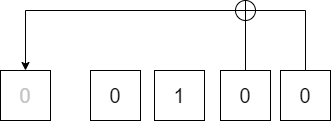
\includegraphics[width=0.5\textwidth,keepaspectratio]{img/lfsr_01.png} .
    \label{fig:mi_imagen}
\end{figure}
\\
En la figura, se aprecia como el XOR entre la posición 0 de la cadena binaria, y la posición 1, resulta en el bit que ocupará la posición 3 de la cadena. Todos los bits del estado anterior se desplazan una posición hacia la derecha eliminando el bit en posicion 0 del estado anterior. Y por último se repite, la operación XOR.
\newpage
\begin{figure}[h] 
    \centering
    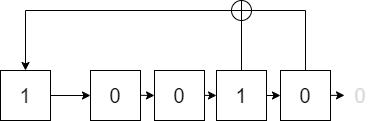
\includegraphics[width=0.5\textwidth,keepaspectratio]{img/lfsr02.png} .
    \label{fig:mi_imagen}
\end{figure}
\noindent El polinomio del LFSR del ejemplo, es un polinomio primmitivo ya que para que el registro vuelva a tener el valor de la semilla es necesario hacer $2^n-1$ iteraciones, ese menos uno se debe a que evidentemente el registro no puede valer 0 ya que en ese caso sin importar el número de iteraciones siempre permanecería en 0.\\\\
Para concluir esta sección y esclarecer del todo este tema de los registro de desplazamiento, en la siguiente figura tenéis un pseudocódigo naive para implementar cualquier LFSR.\\ 
\begin{algorithm}
\caption{Algoritmo lfsr(s, t, k)}\label{alg:zero}
\KwData{$s$ = secuencia binaria, $t$ = lista con las taps positions, k = numero de steps/iteraciones}
\KwResult{s después de k iteraciones}
\For{$i = 0; i < k; i++$}{
    $output \gets s[taps[0]]$\;
    \For{$j = 0; j < len(t); j++$} {
        $output \gets output \oplus s[taps[j]]$\;
    }
    $s = output, s[len(s)-1]$\;
}
\end{algorithm}
\\
Cabe destacar, lo increíblemente simple que es, para lo complejos que pueden llegar a ser los output a los que da salida este algoritmo. Aunque existen técnicas para decodificar estas secuencias y obtener tanto el polinomio como el estado inicial. %La implementación es extremadamente rápida en hardware ya que las operaciones necesarias para generar las secuencias, son dos, desplazamientos y xor. (poner arriba con alguna que otra frase)% \\

\subsection{Fibonacci y Galois}
Hay dos tipos principales de registros de desplazamiento lineal. El que hemos explicado hasta ahora se le denomina LFSR de Fibonacci, aunque este no fuera el autor se le llama así por su relación con las recurrencias. Este tipo de LFSR puede ser de período máximo, es decir si está constituido por un polinomio primitivo, o puede describirlo otro polinomio que no sea primitivo, y entonces tener un período menos a $2^n - 1$. \\\\
El otro tipo es más difícil de explicar y cómo en las siguientes secciones no tiene especial impacto, tan sólo lo mencionaré, se trata del LFSR de Galois (sí, el del duelo y las cartas), en este registro de desplazamiento lineal algunos de los bits se desplazan y otros son el resultado de operaciones entre algunas de las posiciones del propio registro.
\\




\section{Algoritmo de Berlekamp-Massey}
Antes de pasar al algoritmo sobre el que se central de traducción de una secuencia binaria a su FSR mínimo. Debemos explicar el procedimiento que toma como referencia, este es el algoritmo de \textit{Berlekamp Massey}. El algoritmo original, Berlekamp, del que deriva Berlekamp Massey, fue creado para decodificar códigos BCH (Bose-Chaudhuri-Hocquenghem), estos códigos se utilizan para codificar información de manera redundante por si hubiera algún fallo en la transmisión o en el almacenado de los datos poder corregirlos a través de Forward Error Correction (FEC). \\\\
El algoritmo de Berlekamp-Massey, también llamado por su creador James Massey, \textit{LFSR Synthesis Algorithm (Berlekamp iterative algorithm)} en el articulo original \cite{massey1969shift}, es capaz de encontrar la recurrencia lineal más corta para cualquier secuencia numérica finita. Esto tiene mucho que ver con la modificación de este algoritmo que utilizaremos en la siguiente sección para calcular la complejidad no lineal de un secuencia binaria. Además también es el culpable de que el cifrado a través de LFSR sea inseguro, ya que si conoces una parte del texto claro de tamaño suficiente puedes recuperar el \textit{keystream} con el que se cifro.\\\\
Primero explicaré en que consiste el algoritmo para encontrar la recurrencia lineal mas corta para cualquier secuencia de números en base decimal. Dada una secuencia $s = \{s_0, s_1, \dots\}$ diremos que existe una secuencia de recurrencia lineal $c = \{c1, c2, \dots, c_n\}$, las cuales cumplen.
\[s_i = \Sigma_{j=1}^n c_js_{i-j} \quad \text{para $i \geq n$}\]
Para $i \geq n$ tan solo quiere decir que es para todos los números fuera de los casos base ya que los casos base de la recurrencia lineal serán desde $s_0$ hasta $s_n$. Un ejemplo de recurrencia lineal muy típico es la sucesión de Fibonacci o su primo hermana la sucesión de Lucas. \\\\
Berlekamp Massey se basa en lo siguiente. Teniendo una secuencia $s$ cualquiera y una lista con los coeficientes de la recurrencia lineal vacío, ir rellenando la lista de coeficientes según se recorre la secuencia $s$ y en caso de que ocurra un fallo, aplicar una función correctora $d$. También hay que guardar copias de c y tener un índice de un fallo pasado, en el ejemplo veremos para que y por qué.\\\\ 
Veamos esto con un ejemplo sencillo, dada la secuencia $s = \{ 1, 3, 9, 15, 9, -81 \}$ y la la lista $c = \{ \ \}$, asumiremos que si c está vacío, c será igual a 0. Definiremos como $pc$ (\textit{past c}) al conjunto que nos servirá como copia de c, el cual comienza vacío como $c$. Y la variable donde guardaremos el índice al fallo pasado como $f$.
\\\\
En la primera iteración: \\
\(i=0 \quad s_0 = 1 \\
c(0) = 0 \neq s_0\\
f = i = 0
\)\\
Como da igual a que valor pongamos coeficiente añadamos a $c$ ya que $s_0$ ahora será caso base, en mi implementación añado a $c$ tantos ceros como iteraciones hayan pasado hasta el primer fallo en este caso la primera así que $c = \{ 0 \}$.
\\\\
En la segunda iteración: \\
\(i=1 \quad s_1 = 3 \\
c(1) = c_1 * s_{1-1} = 0 \neq s_1\\
\)\\
Al ser el segundo fallo, ya hay que aplicar la función correctora $d$, el cálculo de esta siempre es igual. Primero hacer que $d$ sea igual a $-1 * pc$, insertar un uno en la posición 0 de $d$, multiplicar la secuencia por $\frac{\Delta}{d(f+1)}$, siendo $\Delta$ igual  a $s_i - c(i)$, finalmente debes insertar $i-f-1$ ceros a la izquierda de la lista $c$. En esta iteración $d$ sería igual a. \\\\
\(d = \{ 1 \} \\
 d = \{ 1 \} *  \frac{\Delta}{d(f+1)} \quad \text{siendo} \quad d(i) = \Sigma_{j=1}^n d_js_{i-j} \\
 d(0+1) = 1 \quad \Delta = 3 \quad \frac{\Delta}{d(f+1)} = 3 \\
 d = \{ 1 \} *  \frac{\Delta}{d(f+1)} = 3 \\
 \text{Finalmente, }
 d = \{ 3 \}  \quad \text{ya que, }  \quad i -f -1 = 0
\)\\
Ahora sumamos esta función correctora $d$ a $c$ para obtener nuestra $c$, $c = c + d = \{3\}$. Hay que decir que ni $pc$ ni $f$ han cambiado su valor en esta iteración. Pasaremos directamente a explicar la cuarta iteración (ya que en la tercera no hay fallo) y no repetir los pasos, solamente explicaré el por qué en este fallo sí se actualizan $pc$ y $f$. 
\\\\
En la cuarta iteración: \\
\(i=3 \quad s_3 = 15 \\
c(3) = c_1 * s_{3-1} = 18 \neq s_3\\
\)\\
Tras ejecutar todos los pasos para el cálculo de $d$, queda $d = \{ 0, 0, -12\}$. Y ahora sí que actualizamos tanto $f$ como $pc$.\\\\
\(f = i = 3 \\
pc = c \quad \text{c es la versión de c de $i=2$, es decir, antes de sumar d}\\
\)\\
Esta actualización se debe a que esas variables deben cambiar cuando se cumple $i - len(c) > f - len(pc)$. Intuitivamente, diremos que $pc$ guardará el c con menos coeficientes respecto a donde fallo. \\\\%esto no se como explicarlo bien%
Aquí está el pseudocódigo, podéis encontrar una implementación en Python escrita por mí en \href{https://github.com/domingoUnican/TFGPedroCastro/blob/main/code/code_proofs/simple_berlekamp_massey.py}{simplebm.py} basado en uno de los códigos de \href{https://mzhang2021.github.io/cp-blog/berlekamp-massey/}{artículo berlekamp massey}.



\begin{algorithm}
\caption{Algoritmo Berlekamp-Massey}\label{alg:two}
\KwData{$s$ secuencia binaria}
\KwResult{El LFSR mínimo}
$c \gets [ \ ]$\;
$pc \gets [ \ ]$\;
$f \gets -1$\;
\For{$i = 0; i < len(s); i++$}{
    $delta \gets s[i] - \sum_{j=1}^{len(c)+1}c_{j-1}*s_{i-j}$\;
  \eIf{$f == -1$}{
     $c \gets resize(c, i+1)$\;
     $f \gets i$\Comment*[r]{Para la primera vez}
  }{
  $d \gets - pc$\;
  $d.insert(0,1)$\;
  $df1 \gets \sum_{j=1}^{len(d)}d_{j-1}*s[f+1-j]$\;
  $coeff = \frac{delta}{df1}$\;
  $d \gets d*coeff$\;
  $d \gets \texttt{addzerostoleft(i-f-1, d)}$\Comment*[r]{suma i-f-1 ceros a la izq}
  $copyc \gets c$\;
  \If{\(len(c) > len(d)\)}
  {
   $c \gets \texttt{addzerostoright(len(d) - len(c), d)}$
  }
  $c \gets c + d$\;
  \If{\(i - len(copyc) > f - len(pc)\)} {
        $pc \gets temp$\;
        $f \gets i$\;
    }
  }
}
\end{algorithm}



%NOTA: Se pueden Añadir nota breve de aplicaciones del algoritmo de berlekamp massey


\begin{comment}
Seccion por pulir hasta aclarar el sentido de la diferencia simetrica de conjuntos en este algo
\State $h \gets( \{ a - b + it for it in g \}$
\State $f \gets f \symdif h$
\end{comment}
%\EndIf
%\EndFor
%\EndProcedure
%\end{algorithmic}
%\end{algorithm}
\newpage
\section{Non lineal Feedback Shift Register (NLFSR / FSR)}
NOTA: Puede que sea importante explicar que es, y la conexion con el Lempel Ziv Compression)\\\\
Uno de los objetivos de este proyecto ha sido intentar simplificar la función $h$ resultante del algoritmo del articulo \cite{limniotis2007nonlinear}. El paso previo ha sido analizar y dividir por partes el algoritmo hasta entenderlo completamente, esto ha sido de las cosas que más tiempo me han llevado. \\\\
En esta sección, se tratará de explicar este algoritmo recursivo como a mi me hubiera gustado que me lo explicasen. Este procedimiento toma como base Berlekamp-Massey, el cual resuelve eficientemente el cálculo del LFSR mínimo, y lo adapta para conseguir un registro de desplazamiento no lineal (NLFSR) con un 
polinomio mínimo para una secuencia binaria dada. Se dice que un registro de desplazamiento es no lineal, si en su polinomio se utiliza tanto la operación XOR (suma) como la operación AND (multiplicacion).\\\\
Antes de describir el algoritmo, debo hacer un breve resumen sobre la notación que utilizaré durante esta sección para describir conceptos como una secuencia numérica cualquiera. La notación está basada en la del artículo original. Pero creo que es necesario, plasmarlo aquí, para una mejor lectura de esta parte del trabajo. Para definir un \textit{minterm} usaremos la notación, $\underline{x_b} = x_1^{b1} ,..., x_n^{bn}$, donde $b = (b_1,...,b_n) \in \mathbb{F}_2^{n}$, siendo $x_i^0 = x'_i$ y $x_i^1 = x_i$, por ejemplo, el \textit{minterm} de la secuencia 011 es $x'_1x_2x_3$. Para las cadenas o secuencias, usaré la siguiente notación, diremos que una secuencia binaria de $N$ elementos se escribe $y^{N}$. Si queremos describir un segmento de esa secuencia, escribiremos $y_{i}^{j}$ siendo $i\leq j \leq N-1$. Esto es así porque trataremos las posiciones de las secuencias como si fuesen \textit{arrays} o listas en cualquier lenguaje de programación, es decir, siendo la posición inicial el 0. Definimos la complejidad no lineal de una cadena como $c(y^{N})$. He de decir también que las siglas FSR se utilizaran para referirse al NLFSR (\textit{Non Lineal Feedback Shift Register}). \\\\%(NOTA: puede que queden más cosas, por ahora lo dejo así...)% 
\newpage
Ahora desglosaremos paso por paso el algoritmo y señalaremos las similitudes con Berlekamp-Massey.

\begin{algorithm}
\caption{Algoritmo FSR mínimo}\label{alg:three}
\KwData{$s$ = cadena binaria}
\KwResult{El non linear FSR mínimo}
$k \gets 0$\;
$m \gets 0$\;
$h \gets y_0$\;
\For{$i \gets 1,...,N-1$} {
    $d \gets y_i - h(y_{i-1},\dots,y_{i-m})$\;
    \If{$d \neq 0$} {
    \uIf{$ m = 0 $} {
        $k \gets i$\;
        $m \gets i$\;
    }
    \ElseIf{$k \leq 0$} {
        $t \gets \texttt{Eigenvalue$(y^{i})$}$\;
        \If{$t < i + 1 - m$} {
            $k \gets i + 1 - t - m$\;
            $m \gets i + 1 - t$\;
        }
    }
    $f \gets (x_{1} + y'_{i+1})...(x_m+y'_{i-m})$\;
    $h \gets h + f$\;
    }
    $k \gets k - 1$\;
}
\end{algorithm}

Empezaremos definiendo algunas de las variables y su significado. La variable $k$ está denominada salto y es la distancia entre $c(y^{n})$ y $c(y^{n-1})$. Uno de los teoremas del artículo prueba [X, pp 2] que (falta explicar un poco el por que de esta formula y su relación con $k(y^n)$)
\[k = n - m - (t^{(n-1)}_0 + T^{(n - 1)})\]
Este teorema se usará en el algoritmo para el cálculo del salto. Siendo $t_0^{(n - 1)}$, el preperiodo de la secuencia $y^{n-1}$ y $T^{(n - 1)}$ el periodo de $y^{n-1}$. Es importante aclarar, que $t_0$ y $T$ son el preperiodo y el periodo en el caso de que sean los números enteros más pequeños que cumplan.

\[y_i = y_{i+T} \ \text{para todo} \ i \geq t_0, \text{siendo} \  t_0 \geq 0, T > 0\]
Esto realmente es una forma para los no matemáticos muy enrevesada de decir, que $T$ es la longitud del periodo y $t_0$ el índice en el cual la periodicidad comienza, y a estas dos variables se les llaman \textit{preperiodo} y \textit{periodo}. \\\\
%\href{http://google.com}{Google} ejemplo vinculo

Todo esto será importante, ya que en el caso en el que el salto sea menor o igual que 0, esto podría hacer que la complejidad no lineal de la secuencia cambiara.\\\\
Por otro lado, la variable $m$ es la complejidad no lineal de la secuencia a evaluar. Y h es la función de feedback que acabara generando la secuencia original a partir de un segmento inicial de esa propia secuencia, el núcleo del algoritmo es entender como y por qué se actualiza esta función.\\\\
Pues bien, la clave de todo está en la variable $d$ que se recalcula en cada iteración y que llamaremos \textit{discrepancia}. El cálculo de la \textit{discrepancia} en la iteración $i$ consiste en computar si el resultado de la función de feedback ($h$) de esa iteración difiere de la posición $i$ en la secuencia. En caso de que difiera, se sumará el minterm que hace que esa posición se calcule como corresponde a la función de feedback, actualizando esta última. Cabe destacar, que no porque haya una \textit{discrepancia} tiene que aumentar la complejidad no lineal de la secuencia.\\\\
Existen varios casos si existe una \textit{discrepancia}, el primero de ellos es que aun no se haya inicializado la complejidad no lineal de $y^{n}$, es decir, si m es igual a 0. En ese caso se les asigna tanto al salto, como a $m$ el valor de $n$, es decir la posición de la primera \textit{discrepancia}. Todo esto parece muy complicado pero con el ejemplo al final de la sección, se entenderá mucho mejor. El segundo caso, en el que $m$ no es 0 y $k \leq 0$, se calculará el \textit{eigenvalue} de la secuencia desde la posicion 0 hasta la posicion $n$. Al leer las definiciones de  \textit{eigenvalue} y \textit{eigenwords} en [x], no termine de entender a que se referían, así que fui a la fuente original el artículo \cite{lempel1976complexity}. Esto me ayudo a aclarar los conceptos de vocabulario, prefijos \textit{propios}, \textit{eigenvalues} y \textit{eigenwords} de una cadena $y^n$, junto con otros conceptos como historial, historial exhaustivo, reproducibilidad y producibilidad. \\\\
Vamos a definir brevemente cada una de estas cosas, para entender bien, como y para qué necesita el algoritmo este \textit{eigenvalue}. El vocabulario de una secuencia $y^{N}$ son los subconjuntos de esa misma secuencia formado por todas las \textit{subcadenas} $y_i^{j}$ siendo $0 < i < j$ y $j < N$. Por ejemplo, de esta secuencia 01001, su vocabulario sería.
\[v(y^{N}) = \{0, 1, 01, 10, 00, 01, 010, 100, 001, 0100, 1001, 01001 \}\]
El siguiente paso es encontrar las \textit{eigenwords} (\textit{palabras propias}). Una palabra del vocabulario, es una palabra \textit{propia} si no pertenece a ninguno de los vocabularios de los prefijos propios (\textit{proper} prefixes) de la cadena original ($y^{N}$). Un prefijo \textit{propio} es un segmento desde $i$ hasta $j$, donde $0 < i < j < N-2$, es decir que la longitud del prefijo propio $Q$ debe ser menor que la longitud de la cadena original $y^{N}$, $l(Q) < l(y^{N})$. El conjunto de palabras \textit{propias} se le denomina vocabulario \textit{propio} ($e$)(\textit{eigenvocabulary}). El vocabulario propio del ejemplo anterior sería.
\[e(y^{N}) = \{ 001, 1001, 01001 \}\]
Y ahora ya tenemos la forma de calcular el \textit{eigenvalue} $k(y^N)$, pues el cardinal del vocabulario \textit{propio} es igual al \textit{eigenvalue}, $|e(y^N)| = k(y^N)$, en este caso 3. Toda este proceso tan largo, no es necesario para el calculo del \textit{eigenvalue}, hay una manera mucho más sencilla y óptima, la desarrollaremos un poco más adelante. Podéis consultar una implementación \textit{naive} de este proceso en el programa \href{https://github.com/domingoUnican/TFGPedroCastro/blob/main/code/code_proofs/naive_eigenvalue.py}{naiveEigenvalue.py}.\\\\ Aunque pueda parecerlo, todo este pretexto no es arbitrario, pues con esta explicación tenemos la capacidad de entender, el por qué de la condición en el pseudocódigo, $t < n + 1 - m$. En caso de que la condición, se evalúe como cierta, esto quiere decir que siendo $m = c(y^{n-1})$, $k(y^n) < n - m$. Luego la subcadena de tamaño $m$, $y^{n-2}_{n-m-1}$ se repite dos veces con diferentes sucesores en $y^{n-1}$, esto provoca que se tenga que sumar un \textit{minterm} con una variable más al polinomio, o dicho de otra manera, corregir la función de \textit{feedback}, línea del pseudocódigo \textit{20}. Sin embargo, si la condición se evalúa como falsa, $k(y^{n-1}) >= n - m$, la subcadena $y^{n-2}_{n-m-1}$ ahora es única por lo que a pesar de que se tenga que añadir un nuevo \textit{minterm} a la función de \textit{feedback} el numero de parámetros del polinomio no aumentará, por lo que $c(y^n)$ tampoco. (nota: pordría desarrollar esto un poco mas).\\\\
Hay un punto que hemos pasado por alto, se trata de la función de la variable $k$ (\textit{salto}) en el pseudocódigo. La función principal de esta variable en el algoritmo es ahorrarnos el cálculo del \textit{eigenvalue} en momentos en los que no es necesario calcularlo ya que sabemos que no han pasado suficientes iteraciones como para que pueda haber otro \textbf{salto} en la complejidad no lineal.\\\\
Esta variable solamente condiciona el flujo del programa en el \textit{if} $k <= 0$, y como se puede observar se resta 1 a esta variable por iteración, y cuando es menor o igual a 0, se le asigna la diferencia entre $c(y^n)$ y $c(y^{n-1})$. Esto en realidad, se hace para que tengan que pasar $c(y^n) - c(y^{n-1})$ iteraciones, hasta que pueda darse un nuevo salto en la complejidad ya que a partir de esas iteraciones es cuando \textbf{podrían} aparecer 2 subcadenas de longitud $m$ con diferentes sucesores, es en ese momento donde el cálculo del \textit{eigenvalue} cobra relevancia.\\\\
Con todo este conocimiento previo, vamos a analizar un ejemplo en el que iremos explicando paso a paso, que hace el algoritmo. Tomando la secuencia binaria $y^{10} = 1101010011$, antes de entrar al bucle $k$ y $m$ serán 0. Y $h(x) = y_0 = 1$, téngase en cuenta que al contador/iterador lo llamaremos $i$ por comodidad. \\\\
En la primera iteración del bucle: \\
\(i=1 \quad y_1 = 1 \\
\text{Calculo de la discrepancia de $y^1 = 11$:}\\
\text{$h(1) = 1$, en este momento, h(x) es una función constante}\\
\text{¿es $h(1)$ igual a $y_1$?, sí, por lo que no hay discrepancia}\\
\text{$k = k - 1$, y seguimos adelante}
\)\\\\
En la segunda iteración del bucle: \\
\(i=2 \quad y_2 = 0 \\
\text{Calculo de la discrepancia de $y^2 = 110$:}\\
\text{$h(1) = 1$, h(x) sigue siendo una función constante}\\
\text{¿es $h(1)$ igual a $y_2$?, No, así que tenemos nuestra primera \textbf{discrepancia}}\\
\text{Al ser la primera discrepancia, $m = 0$, así que}\\
m = i  \quad k = i \\
\text{\textbf{Importante}, toca corregir nuestra función \textit{fsr}, añadiendo el \textit{minterm}} \\
\underline{x_{\{ 11 \}}} = x_0*x_1 \\
h(x) = h(x) + \underline{x_{\{ 11 \}}} = 1 + x_0*x_1 \\ 
\text{Y como en todas las iteraciones, }\\
\text{$k = k - 1$}
\)\\\\
Antes  pasar a la siguiente iteración, quería hacer un apunte, parece una tontería pero es que gracias al evaluar la función en modulo 2. Es muy simple e intuitivo que al añadir el \textit{minterm} de esa posición, la función se corrija. Ya que si antes te daba 1, con el \textit{minterm} (pues el minterm equivale a 1, en esa posicion de la cadena) cambiará a 0, y viceversa.\\\\
En la tercera iteración del bucle: \\
\(i=3 \quad y_3 = 1 \\
\text{Calculo de la discrepancia de $y^3 = 1101$:}\\
\text{La subcadena que servirá como input hay que darle la vuelta para que coinci- }\\
\text{da con el orden de las variables.}\\
y^{3-1}_{3-m} = y^2_{1} = 10 \\
\texttt{reverse($y^2_{1}$) = 01} \\
h(x_0=0, x_1=1) = 1+0*1 = 1\\
\text{¿es $h(01)$ igual a $y_3$?, Sí, no se realizan cambios en $h(x)$}\\
\text{$k = k - 1$}                      
\)\\\\
\\\\
En la cuarta iteración ocurre una \textit{discrepancia} que no cambia la complejidad no lineal $m = c(y^n)$, tan solo añade a la función $h$ el \textit{minterm}, $x_0*x'_1$. En la quinta y sexta no hay discrepancias. Sin embargo, en la séptima iteración ocurre lo siguiente\\\\
\(i=7 \quad y_7 = 0 \\
\text{Calculo de la discrepancia de $y^7 = 11010100$:}\\
y^{7-1}_{7-m} = y^6_{5} = 10 \\
\texttt{reverse($y^6_{5}$) = 01} \\
h(x_0=0, x_1=1) = 1+0*1+0*(1+1) = 1\\
\text{¿es $h(01)$ igual a $y_7$?, No}\\
\)\\
Ya que hay más de una subcadena $y^{i-1}_{i-m}$ con distintos sucesores, hay que aumentar la complejidad no lineal $m$, en concreto $y^6_{5}$ se repite 2 veces previamente pero con el mismo sucesor. En esta iteración es la tercera vez que se repite la subcadena pero se da una discrepancia. 
\[
{\text{\large $10 \quad \textcolor{green}{\xrightarrow{}} \quad 10 \quad \textcolor{green}{\xrightarrow{}} \quad 10 \quad \textcolor{red}{\xrightarrow{}} \quad 0$}}
\]
Al darse este caso, el \textit{eigenvalue} será menor que $n + 1 - m$. Por lo que se actualizará el $k$ y $m$. \\
\(
k = n + 1 - t - m \\
m = n + 1 - t \\
\text{El siguiente paso es sumar el \textit{minterm} con $m$ ya actualizada, por lo que }\\
\underline{x_{\{ 01010 \}}} = x'_0*x_1*x'_2*x_3*x'_4 \\
h(x) = h(x) + \underline{x_{\{ 01010 \}}} = 1 + x_0*x_1 + x_0*x'_1 + x'_0*x_1*x'_2*x_3*x'_4\\ 
\text{Y al final de la iteracion, }\\
k = k - 1                     
\)\\\\
(Falta una pequeña explicacion de por k = n + 1 - t -m y m = n + 1 - t)\\
En la octava iteración no se dan discrepancias. Y por último, en la novena se da una discrepancia que no aumenta $m$, sumando el minterm $x_0*x'_1*x'_2*x_3*x'_4$. Aquí termina el ejemplo, habiendo recorrido toda la cadena, y quedando una función final de feedback tal que así 
\[h(x) = 1 + x_0*x_1 + x_0*x'_1 + x'_0*x_1*x'_2*x_3*x'_4 + x_0*x'_1*x'_2*x_3*x'_4 \]
Con esta función podríamos a partir de los primeros 5 digitos de la secuencia recuperar la secuencia entera, aplicando la función de feedback, añadiendo el resultado a la derecha y recalculando. Este proceso debe repetirse, siendo $w$, el numero de parámetros de la función de feedback y $r$, la longitud original de la cadena. Se aplicará el proceso $r - w$ veces, para conseguir la secuencia original. Podéis consultar también el decodificador, que he escrito en Python en \href{https://github.com/domingoUnican/TFGPedroCastro/blob/main/code/common/utils.py}{verificamfsr.py}. 

\subsection{Como encontrar el \textit{eigenvalue} de manera óptima}
Esta métrica es esencial en nuestro algoritmo previo, y ya hemos descrito anteriormente como calcularla de la manera más sencilla o "\textit{naive}". Sin embargo, en el articulo original \cite{limniotis2007nonlinear} en la sección que describe el procedimiento recursivo, indican que la manera más eficiente de calcular el \textit{eigenvalue}, es mediante el algoritmo de \textit{Knuth Morris Pratt}. Este algoritmo nos permite buscar con una complejidad temporal muy buena, un patrón en una cadena a la que cual llamaremos texto. \\\\
El algoritmo consta de dos partes, la primera, la llamaremos \textit{preprocesado}, la cual tiene una complejidad temporal $O(m)$, siendo $m$ la longitud del patrón. En esta sección, se calcula una tabla a la que normalmente se le llama \textit{longest proper boundary table}. Esta tabla, en términos prácticos, será una lista en la que cada posición indica el \textit{longest proper boundary} de la secuencia hasta ese carácter o dígito dependiendo del tipo de cadena a la que le apliquemos el algoritmo. Este valor, representa el tamaño de la subcadena más larga que es a la vez prefijo y sufijo de la cadena hasta el índice de esa posición del patrón. Esta tabla o lista, después nos ayudará en la segunda parte del algoritmo pues a \textit{grosso modo}, nos permitirá "recordar" que parte del patrón nos coincide en cada iteración.\\\\
En la segunda parte, recorremos el texto, ese bucle evidentemente tendrá complejidad $O(n)$, siendo $n$ la longitud del texto. Y lo que haremos, en realidad, es bastante simple, se recorre el texto y el patrón a la vez con dos índices distintos, $i$ para el texto y $j$ para el patrón, mientras los caracteres del texto y del patrón coincidan, ambos avanzan a la misma velocidad. Pero, cuando no coinciden si el patrón ha coincidido parcialmente con la parte del texto que se itera en ese momento, entonces es cuando entra la lista $lpb^m$ en acción. Ya que, se le asignará al índice el valor de $lpb_{j - 1}$, y  no aumentará $i$ en esa iteración. Retrocediendo el índice del patrón hasta $lpb_{j-1}$, lo que se consigue es ahorrar en iteraciones pues a pesar de que no haya coincido en ese carácter puede que coincida más atrás del patrón. En el caso, de que el patrón coincida completamente en el texto, el índice $j$ se le asigna $lpb_{m-1}$, puesto que la cuenta de coincidencia del patrón puede empezar en el índice $lpb_{m-1}$.\\\\
A continuación, tenéis una implementación general de este algoritmo, que devuelve si el patrón se encuentra o no en el texto, no es difícil imaginar que también puedes devolver el numero de coincidencias del patrón en el texto, que es justo lo que nos interesa para el \textit{eigenvalue}.\\\\
\newpage
\begin{algorithm}
\caption{Algoritmo KMP (Knuth Morris Pratt)}\label{alg:four}
\KwData{$s$ = cadena binaria}
\KwResult{True si encuentra el patrón False si no lo encuentra}
$n \gets len(t)$\;
$m \gets len(p)$\;
\tcc{Preprocesado, calculo de lpb}
$lpb \gets (0)_m$\;
\For{$i = 0; i < m; i++$} {
    $j \gets lpb_{i-1}$\;
    \While{$j > 0 \And p_j \neq p_i$} {
        $j \gets lpb_{j-1}$\;
        \eIf{\(p_j == p_i\)} {
            $lpb_i \gets j+1$\;
        }
        {
        $lpb_i \gets j$\;
        }
    }
}
\tcc{Busqueda de p en t}
$isFound \gets false$\;
$j \gets 0$\;
\For{$i = 0; i < n; i++$}{
    \While{\(j > 0 \And t_i \neq p_j\)} {
        $j \gets lpb_{j-1}$\;
    }
\If{\(t_i == p_j\)} {
    $j \gets j + 1$\;
}
\If{\(j == m\)} {
    $isFound \gets true$\;
    break\;
    \tcc{Si no se para despues de la primera coincidencia completa}
    \tcc{ $j \gets lpb_{j-1}$}
    }

}
\texttt{return} $isFound$\;
\end{algorithm}
La tabla de debajo de este párrafo se ha tomado de \cite{leiserson2022introduction}, un libro donde explican en detalle y con claridad todos estos algoritmos de búsqueda en cadenas. Lo destacable de esta tarde es la notoria diferencia entre \textit{Knuth Morris Pratt} y el \textit{Naive}, este \textit{Naive} recorre la cadena buscando el patrón y cada vez que un carácter del patrón no le coincide, reinicia la búsqueda desde el siguiente carácter es por esto por lo que nos da una complejidad de $O((n-m+1)m)$. 
\begin{center}
\begin{tabular}{ l c c }
 Algortimo & Tiempo de Preprocesado & Tiempo de ejecución \\ \cline{1-3}
 Naive & 0 & $O((n-m+1)m)$ \\  
 Rabin-Karp & $O(m)$ & $O((n-m+1)m)$ \\
 Automáta finito & $O(m|\Sigma|)$ & $O(n)$ \\
 Knuth Morris Pratt & $O(m)$ & $O(n)$
\end{tabular}
\end{center}

Nosotros aplicaremos este algoritmo para encontrar el \textit{eigenvalue} de la siguiente manera en la función \textit{Eigenvalue} del pseudocódigo. Guardaremos en una variable $p$ (patrón), la cadena \texttt{reverse($y_0^{i-1}$)}, y en otra variable $t$ (texto), la cadena $p_1^{i-1}$. Y teniendo una función \textit{knuthmp} implementada con \textit{Knuth Morris Pratt}, que podéis consultar en \href{https://github.com/domingoUnican/TFGPedroCastro/blob/main/code/minimal_fsr/knuthMorrisPratt.py}{kmp.py}, que lo que hace es devolver el numero de posiciones que se encuentran del patrón en el texto. Devolveremos
\[Eigenvalue(y^i) = i - knuthmp(t, s)\]
Esta diferencia puede dar como resultado un numero en el intervalo $[1, i]$ en función del numero de coincidencias del patrón.


\section{Formato de archivo nlfsr}
El formato de archivo nlfsr (Non Linear Feedback Shift Register) es un formato el cual codifica la secuencia inicial y el polinomio FSR. Teniendo como objetivo hacer que este tipo de archivo ocupe el menor espacio posible, para ello he propuesto que la estructura del formato fuera la siguiente.
\\
\begin{figure}[h] 
    \centering
    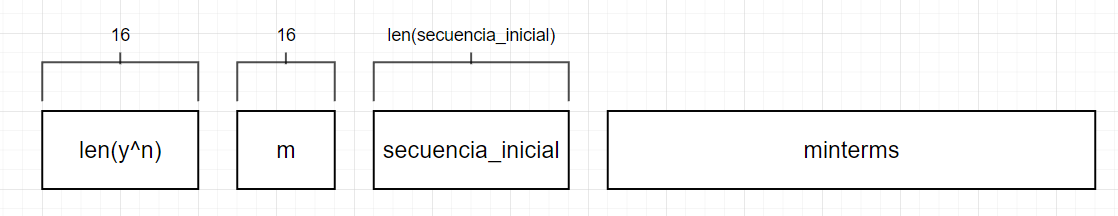
\includegraphics[width=\textwidth,keepaspectratio]{img/nlfsrformat_01.png} .
    \parbox{\linewidth}{\centering Formato .nlfsr}
    \label{fig:mi_imagen}
\end{figure}

\noindent El primer segmento del archivo es la longitud de la cadena original ($y^n$), contenido en 16 bits. Estos 16 bits limitan el tamaño de la secuencia a comprimir en este formato, a una secuencia de longitud máxima 65536. Este límite es arbitrario, pero una vez se haya leído toda la explicación del formato entenderéis que no es difícil adaptarlo para cadenas más largas.  El segundo segmento es la complejidad no lineal $m$ de $y^n$ contenida también en 16 bits (o 2 Bytes). El tercer segmento es la secuencia inicial que mide $m$ bits. Y el cuarto segmento es una lista de \textit{minterms}, aquí tenéis una representación de como se representa un \textit{minterm}.
\\
\begin{figure}[h] % El [H] asegura que la imagen esté exactamente en ese lugar en el documento.
    \centering
    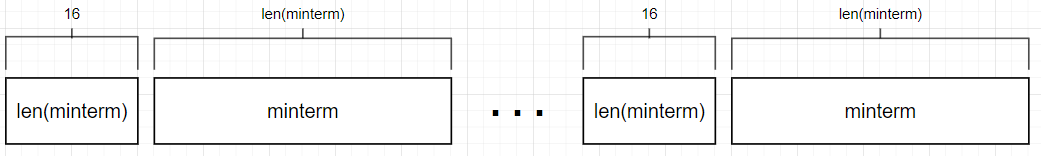
\includegraphics[width=\textwidth,keepaspectratio]{img/nlfsrformat_02.png} % La imagen se ajustará al ancho del texto, manteniendo la proporción.
    \parbox{\linewidth}{\centering Lista de minterms en formato .nlfsr}
    \label{fig:mi_imagen} % Etiqueta para referenciar la imagen en el documento.
\end{figure}
\noindent Cada \textit{minterm} consta de un primer segmento en el que se indica el numero de variables de ese producto de literales lógicos, o dicho de otra manera la longitud. Cada bit del \textit{minterm} representara el estado de ese literal en el producto, si su valor es 1 eso significa que el literal se encuentra negado, por otro lado, si es 0, significará que es positivo. De esta manera, conseguimos almacenar toda la información consumiendo el mínimo numero de bytes posibles. \\\\
La longitud del propio \textit{minterm} actuando como delimitador entre \textit{minterms}, nos permite saber hasta donde tenemos que leer cuando haya que decodificar el archivo .nlfsr. Es importante aclarar, que no se pueden utilizar delimitadores fijos en este caso, como sí se en algunos protocolos de red, ya que toda secuencia podría estar dentro del minterm, y eso haría que se mezclasen los datos con las delimitaciones, lo cual provocaría errores en el momento de la lectura.
\\\\
He hecho unas gráficas para que se pueda ver la diferencia entre guardar un nlfsr de una secuencia con la misma estructura del formato .nlfsr pero usando caracteres ASCII, y utilizar el formato .nlfsr. Aquí tenéis las gráficas sin que se haya utilizado ningún algoritmo de compresión después. 
\begin{figure}[h] % El [H] asegura que la imagen esté exactamente en ese lugar en el documento.
    \centering
    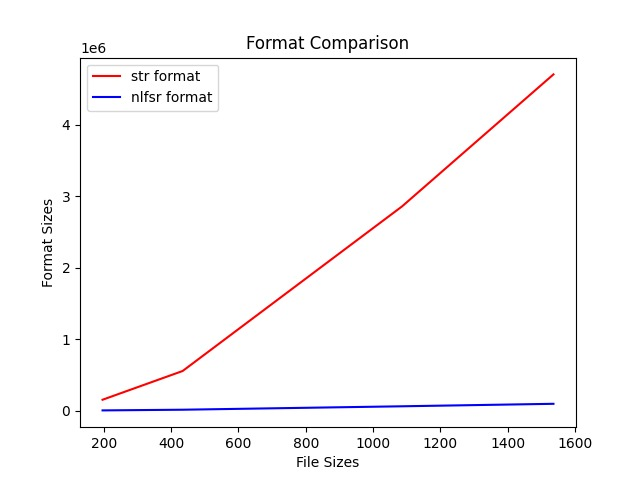
\includegraphics[width=0.8\textwidth,keepaspectratio]{img/format_comparison_graph.jpeg}
    \parbox{\linewidth}{\centering Comparación tamaños formatos}
    \label{fig:mi_imagen} 
\end{figure}
%Encriptación distribuida,
% \subsection{Potenciales aplicaciones del formato nlfsr} (posible seccion)
% Encriptación minimizada distribuida,
\newpage
\section{Minimización de ESOP}
La minimización de expresiones de operaciones AND-OR cuenta con muchos algoritmos que hacen un buen trabajo, sin embargo la minimización de ESOP resulta ser mucho más compleja o al menos, no se han desarrollado algoritmos del mismo calibre. Pero primero, definamos que es todo esto.\\\\
A la forma de la función FSR, se la conoce como ESOP (\textit{Exclusive Sum Of Products}). Una formula lógica con esta forma, tan solo puede tener dos operaciones: XOR (suma) y AND (multiplicación). Minimizar una fórmula ESOP, significa encontrar una formula de menor tamaño que tenga la misma tabla de verdad, o el mismo mapa de Karnaugh; en definitiva, que sean equivalentes.Aquí tenéis un ejemplo de un ESOP y su minimización, aunque más tarde veremos la teoría que hay detrás.
\\\\
\noindent
\begin{minipage}{0.5\textwidth}
    \centering
    \begin{karnaugh-map}[4][2][1][$X_1X_0$][$X_2$]
        \minterms{1, 5, 6, 7}
        \maxterms{0, 2, 3, 4}
    \end{karnaugh-map}
\end{minipage}
\begin{minipage}{0.5\textwidth}
    \[
    f(X_0, X_1, X_2) = X_0X_1 \oplus X_1X_2 \oplus X_2
    \]
\end{minipage}%
\\
Ahora trataremos de encontrar una equivalencia entre $X_1X_2 \oplus X_2$ y un cubo formado por estos literales. Encontramos que
\\\\
\noindent
\begin{minipage}{0.5\textwidth}
    \centering
    \begin{karnaugh-map}[2][2][1][$X_1$][$X_2$]
        \minterms{1}
        \maxterms{0,2, 3}
    \end{karnaugh-map}
\end{minipage}
\begin{minipage}{0.5\textwidth}

     \begin{align*}
          f'(X_1, X_2) =  X_1X_2 \oplus X_2 \\
     z(X_1, X_2) =  X'_1X_2 \\
     f' = z
     \end{align*}
\end{minipage}%
%\newpage
Y sabiendo esto, sustituimos en la formula original y nos queda un ESOP minimizado

\[f_{min} = X_0X_1 \oplus X'_1X_2\]
\\
La \textit{Suma Exclusiva de Productos} se ha estudiado desde 1925 [Paper original], el artículo más reciente que he encontrado respecto a este tema es []. En este describen un algoritmo en el que mediante transformaciones de cubos, expresiones pseudokronecker, reescritura de términos \cite{brand1993minimization}, y estructuras de datos como BDD (Binary Decision Diagram). Nuestra aproximación al problema en este proyecto será mucho más sencilla pero haber leído todos estos artículos sobre el tema, me ha hecho entender más en profundidad lo complejo que es.
\\\\
A pesar de no hacer una implementación como la de [Heuristic Minimiza], en esta sección tomaremos prestada la teoría que elabora el artículo sobre los cubos que forman los ESOP. Definiremos como "cubo" a cada producto del ESOP. Definiremos como distancia entre cubos, el numero de variables que aparecen de distinta "forma" respecto al otro cubo. Una variable puede aparecer en un cubo de tres maneras: en positivo, negada, o no aparecer. Por ejemplo, un cubo $ab$ tiene distancia 1 respecto a un cubo $ab'$. Lo último, que creo que se debe tener en cuenta del articulo para la posible mejora de nuestro algoritmo, son dos proposiciones 
\begin{tcolorbox}
\textbf{Proposición 1:}\\
Si añades el mismo cubo dos veces a cualquier ESOP, la función no cambiará. \\
\textbf{Proposición 2:}\\
La suma de dos cubos con distancia 1 se puede representar en un solo cubo. 
\end{tcolorbox}
%\noindent En el ejemplo anterior aplicamos la segunda proposición para minimizar la función.





\subsection{Enumeración explicita para encontrar el ESOP de N variables de menor longitud}
¿Y si en lugar de encontrar el mínimo para una fórmula en concreto, encontramos el mínimo de símbolos que debe de tener una fórmula para todos los resultados posibles dada una formula (o ESOP) de n variables de entrada? Pues bien, esto es justo lo que hace nuestro pequeño algoritmo. En lo que sigue veremos paso a paso en que consiste. El primer paso que debemos entender es como conseguimos representar todas las formulas posibles de n variables con m simbolos, pudiendo ser cada símbolo, o bien, un XOR, o bien, un AND. La estructura que utilizamos para lograrlo es muy sencilla, es una lista de enteros. Pero tiene un truco, y es que el 0 representa el XOR o la suma, el 1 representa la operación AND o la multiplicación, y el 2 representa la negación. Cualquier entero $i > 2$ representa una variable de entrada $X_{i - 3}$. Con este sistema de representación en el que cualquier fórmula puede ser representada por una lista o cadena de enteros en la que cada posición tiene un entero $i$, $0 <= i < n+3$ de longitud, $m+(m+1)$, siendo $n$ el numero de variables de la fórmula y $m$, el numero de símbolos(XOR, AND) que puede tener la fórmula. \\\\
Para entender mejor el sistema, pondré los siguientes ejemplos. Teniendo una formula $X_0 * X_2 * X_3 + X_0$ y otra formula $X'_0 + X_1 * X_3 + X_4$, estas son sus representaciones con este sistema.
\begin{align*}
X_0 * X_2 * X_3 + X_0 = [0, 1, 3, 1, 5, 6, 3] \\
X'_0 + X_1 * X_3 + X_4 = [1, 0, 2, 3, 4, 0, 6, 7]
\end{align*}
El cálculo del numero de posibles resultados para una formula de n variables de entrada es
\[k = 2^{2^{n}}\]
Ahora debemos encontrar para cada posible resultado del conjunto de posibles resultados de tamaño k, una formula que satisfaga ese resultado. Para ello lo que haremos, será generar todas las combinaciones con repetición del conjunto $\{0,1, ..., n + 3 - 1\}$ de longitud $p$, definimos al conjunto de todas las combinaciones como $g^{(n+3-1)^p}$, cada elemento de $g$ será una posible combinación de tamaño $p$. Es importante decir que, $p$ determinará el numero de posibles símbolos que pueden haber en la fórmula. \\\\
\newpage
Es cierto que habrá algunas combinaciones que no tendrán sentido sintáctico en esta gramática que hemos creado. Por ejemplo $[2, 2, 2, 2, 2, 2, 2]$, no representa ninguna fórmula. Para distinguir entre las listas que tienen sentido de las que no, hemos escrito una función recursiva que crea una cadena de texto o \textit{string} en base a la lista. Aquí tenéis el pseudocódigo, también podéis leer el código real escrito en Python en \href{https://github.com/domingoUnican/TFGPedroCastro/blob/main/code/logicformula_solver/logicform_solver.py}{logicformulasolver.py}.
\begin{algorithm}
\caption{Algoritmo intListToStringFormula(f)}\label{alg:five}
\KwData{$f$ = lista de enteros}
\KwResult{Función lógica en formato string}
\If{\texttt{isNotEmpty(f)}} {
    $val \gets \texttt{f.pop()}$\tcp*{pops last int from f}
    
    \If{\(val == 0\)} {
        \texttt{return stringFormula(f) + '+' + stringFormula(f)}\;
    }
    \If{\(val == 1\)} {
        \texttt{return stringFormula(f) + '*' + stringFormula(f)}\;
    }
    \If{\(val == 2\)} {
        \texttt{return 'not' + stringFormula(f)}\;
    }
    \texttt{return 'x' + (val - 3)}\;
}
\texttt{return 'S'}\;
\end{algorithm}

\noindent El siguiente paso, es escribir la función para calcular cuantos posibles resultados se generan para un numero de variables dado y una longitud de la cadena de lista de enteros dada. Que lo único que hace es para cada cadena de enteros válida (validada con la función del pseudocódigo escrita encima de este párrafo). Prueba todas las posibles combinaciones de las variables de entrada de la función, es decir si por ejemplo, es una función de 3 variables de entrada probara las $2^3$ combinaciones. Recopilará todos los resultados y hará una lista con ellos. La intentará sumar a un set, la cual se sumará en función del hash calculado a esa lista internamente por Python.\\\\ Una vez se han agotado todas las combinaciones de listas de enteros ("formulas lógicas"), se comparará la longitud del set con el número de posibles resultados $k$; si estos coinciden es que hemos encontrado el tamaño mínimo de la lista de enteros para generar todas las formulas necesarias que coinciden con todos los resultados posibles. \\ 
\newpage
\noindent Aquí tenéis dos gráficas creadas con la librería \textit{matplotlib}, en el eje $X$ la primera fila es el tiempo que ha tardado en ejecutar el algoritmo, y la segunda fila es el tamaño de la lista de enteros. El eje $Y$ representa el numero de posibles resultados retornados por el algoritmo.

\begin{figure}[h!]
    \centering
    \begin{minipage}{0.5\textwidth}
        \centering
        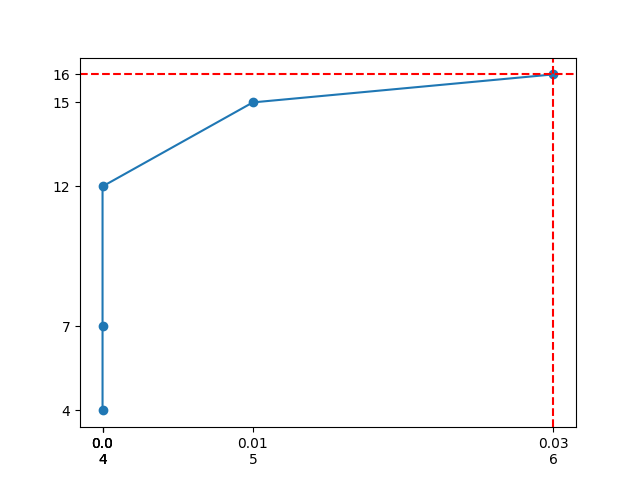
\includegraphics[width=\linewidth]{img/2_variables.png}
        \parbox{\linewidth}{\centering ESOP de 2 variables de entrada}
    \end{minipage}%
    \begin{minipage}{0.5\textwidth}
        \centering
        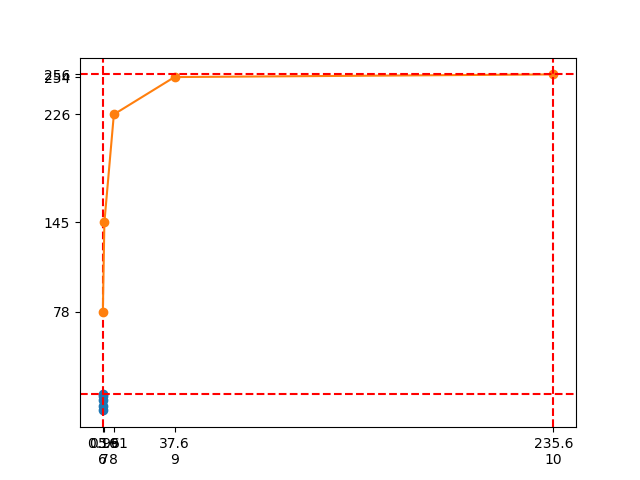
\includegraphics[width=\linewidth]{img/3_variables.png}
        \parbox{\linewidth}{\centering ESOP de 3 variables de entrada}
    \end{minipage}
    \vspace{1em} % Espacio entre las filas de imágenes

    \begin{minipage}{0.5\textwidth}
        \centering
        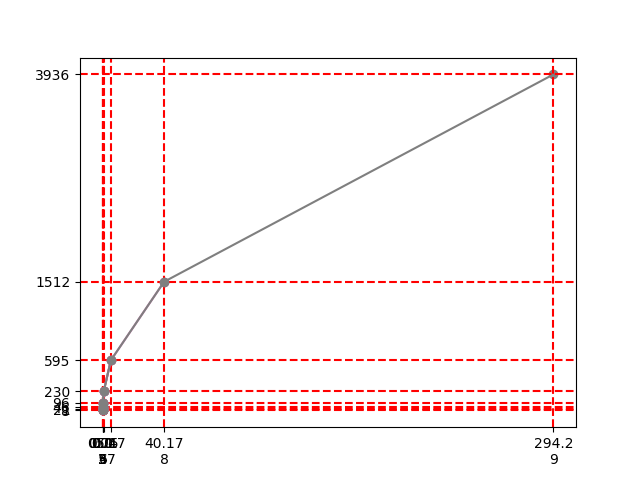
\includegraphics[width=\linewidth]{img/4_variables.png}
        \parbox{\linewidth}{\centering ESOP de 4 variables de entrada}
    \end{minipage}
\end{figure}

\noindent Como vemos en las gráficas, el algoritmo converge en ambos casos es decir, encuentra todas las listas de enteros que satisfacen los $k$ posibles resultados para ESOP de $n$ variables. Sin embargo, a partir de ESOPs de 4 variables debido a la complejidad temporal del algoritmo, se tarda mucho en que el algoritmo converja y empeora conforme el número de variables aumenta, ya que la complejidad temporal de nuestro algoritmo es de $O((n+3)^p * 2^n)$. Con mi procesador, en 10 minutos consigue calcular la función hasta $p = 9$.
\\\\
Para calcular las combinaciones en el código original, hemos usado la librería \textit{itertools}, y en concreto la función \textit{product}, ya que fue una recomendación de mi tutor, Domingo. Este modulo de Python genera sus funciones, utilizando Cython para después crear módulos utilizables desde Python, pero escritos en C. Sentí cierta curiosidad, por como sería hacer un programa en C que calcule todas las combinaciones tal y como lo hace \textit{itertools}.\\\\
Así que me puse manos a la obra, y escribí dos versiones una secuencial \href{https://github.com/domingoUnican/TFGPedroCastro/blob/main/code/list_product/list_product.c}{secuencial.c}. y otra paralelizada con \textit{OpenMP} \href{https://github.com/domingoUnican/TFGPedroCastro/blob/main/code/list_product/list_product_parallel.c}{paralelo.c}. Si habéis leído el código sabréis que lo hago todo sobre un solo array, lo escribí así por temas de la localidad de los valores guardados. En mi \textit{hardware}, el código secuencial resultó ser un poco más lento que el de \textit{itertools}, sin embargo, para mi sorpresa el código paralelizado sí me dio mejores resultados, incluso superando a la función del módulo de Python. Si bien, es cierto que Python está "capado" por el GIL (Global Interpreter Locker), ya que a pesar de contar con módulos que ofrecen funciones de "multithreading" no se consigue en ningún momento una paralelización real, considero que los datos siguen siendo interesantes, aquí tenéis una gráfica.

\begin{figure}[h] % El [H] asegura que la imagen esté exactamente en ese lugar en el documento.
    \centering
    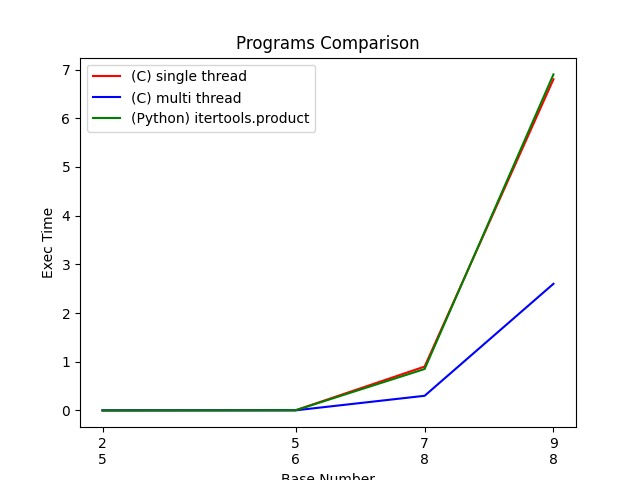
\includegraphics[width=0.9\textwidth,keepaspectratio]{img/programs_comparison_graph.jpeg}
    \parbox{\linewidth}{\centering Comparación tamaños formatos}
    \label{fig:mi_imagen} 
\end{figure}
\noindent El eje Y es el tiempo de ejecución en segundos, y el eje X tiene 2 listas de valores, la lista más cercana al eje es el cardinal del conjunto sobre el que se calculan todas las posibles combinaciones. y el tamaño de la lista es el número de debajo. Cabe destacar que para un conjunto de 10 elementos y un tamaño de lista 8, mi sistema operativo (Debian \textit{bookworm}) mataba el proceso de Python. Sin embargo, para los mismos parámetros mis programas escritos en C, tanto el secuencial como el paralelo, registraron 16.8 y 5.8 segundos respectivamente. Evidentemente con parámetros más altos tenía problemas de memoria debido a mi \textit{hardware} limitado.



\chapter{Conclusiones y posibles avances futuros}\label{cap:Conclusiones}
\section{Avances futuros}
En este trabajo se tocan muchos temas distintos. Cada uno de ellos puede expandirse mucho más de lo que se ha hecho aquí. Se me ocurren muchas posibilidades para expandir GoneFSR y la investigación de la minimización de ESOP (\textit{Exclusive Sum of Products}), a continuación enumeraré algunas de ellas.\\\\
Para el compilador GoneFSR se podría trabajar en implementar operadores lógicos \textit{bitwise}, implementar instrucciones de control de flujo como \textit{break} o \textit{continue}. O en funcionalidades más complejas, como implementar paradigmas como OOP (\textit{Object Oriented Programming}) con sus respectivas clases, atributos y demás. Podría parecer complicado, pero creo que no lo es tanto ya que las clases no dejan de ser funciones, las cuales tienen otras funciones definidas dentro de su \textit{scope}. En un futuro, también me gustaría programar algún sistema de importaciones para poder trabajar sobre varios ficheros, teniendo en cuenta las importaciones circulares y otras casuísticas. Otra futura implementación podría ser la mejora en la administración de memoria con sistemas como la \textit{garbage collection} de Python que a partir de técnicas como el conteo de referencias, o el \textit{cycle detection} para evitar ciclos de referencias, gestionan la liberación de la memoria de las variables a las que no se hace referencia. Y por qué no, puestos a imaginar un gestor de módulos como \textit{pip} o \textit{npm}.\\\\
Por otro lado, se podría desarrollar un backend personalizado con optimizaciones de código usando vectorización con instrucciones SIMD (\textit{Single Instruction Multiple Data}), \textit{unrolling} para descomponer bucles y aumentar la paralelización del código, reordenación de instrucciones para minimizar tiempos de espera. Estas son sólo unas pocas líneas de investigación que se pueden seguir en el desarrollo de un backend de compilación.\\\\
En cuanto a la segunda parte del proyecto hay muchas cosas que he estado estudiando antes de escribir esta memoria que no han podido ser reflejadas en estas líneas ya que a pesar de que puede que tengan que ver, quedaban fuera de los límites del proyecto. Como por ejemplo conceptos como la síntesis de programación, la cual trata de generar programas que cumplan ciertos requisitos, estudiando algoritmos como la enumeración explicita e implícita, si queréis saber más podéis consultar estos artículos \href{https://people.csail.mit.edu/asolar/SynthesisCourse/Lecture1.htm}{\textit{programming synthesis}}. O novedosos avances del estado del arte de la inteligencia artificial, como los sistemas de agentes LLM (\textit{Large Language Model}) (p.ej \cite{islam2024mapcoder}) para generar programas con tan sólo una vaga descripción de lo requerido.\\\\
Donde más potencial de investigación en lo referido a las funciones de registro de desplazamiento estudiadas creo que existe es en la minimización de ESOP, destiné algún tiempo a estudiar el artículo \cite{mishchenko2001fast} y a estudiar código que encontre de su proyecto \textit{EXORCISM} para minimizar estas funciones lógicas. Me estaba llevando mucho tiempo y no conseguí llegar a nada en concreto, pero creo que con el suficiente tiempo se puede indagar en ese campo para buscar nuevas optimizaciones. Creo que otra aproximación adecuada para este problema de minimización podrían ser los SMT (\textit{Satisfacibility Modulo Theories}) como \textit{Z3}, y los SAT solvers, que hace relativamente poco consiguieron resolver el teorema de las tripletas booleanas pitagóricas en 4 años de CPU tal y como dice el matemático Terrence Tao en la \href{https://www.youtube.com/watch?v=e049IoFBnLA&t=1061s}{conferencia}.
\section{Conclusión}
Este proyecto ha llevado mucho trabajo, ha habido momentos muy frustrantes tanto en el desarrollo del compilador, como en la investigación de los algoritmos de registro de desplazamiento. Pero no me arrepiento en absoluto de haberme embarcado en esta empresa. \\\\
La implementación de las sentencias condicionales, trabajar con strings en llvm, añadir la capacidad de escribir funciones, parece poco pero son muchos problemas distintos a los que enfrentarse. Aunque es cierto, que una vez entiendes la estructura central del compilador cada extensión no es tan complicada pues al final son modificaciones de esa propia estructura.\\\\
Entender como funciona el algoritmo de la sección \ref{nlfsr algorithm} me llevo mucho tiempo, entender por qué se suma los minterms como se suman, el por qué del cálculo del \textit{eigenvalue}, conceptos como la complejidad de \textit{Lempel-Ziv} u otros de los que nunca había oído hablar. Intentar hacer un formato que sea óptimo para guardar la información de ese algoritmo. Todo esto fue como hacer un \textit{puzzle} en el que te dan las piezas pero no sabes cómo es la imagen final que deben de formar.\\\\
A modo de conclusión final, me gustaría reafirmar que este proceso aunque haya tenido sus malos ratos y sus momentos de satisfacción cuando todo cuadraba (o cuando parecía que todo cuadraba y al final no), creo que ha merecido la pena, y acabo el proyecto siendo un mejor ingeniero informático.



% Indique aquí el fichero .bib que contenga su bibliografía.
\bibliography{refs}

\appendix
\chapter{Apéndice 1: Gramática completa }
\label{apéndice 1}
\begin{figure}[h!]
  \begin{center}
    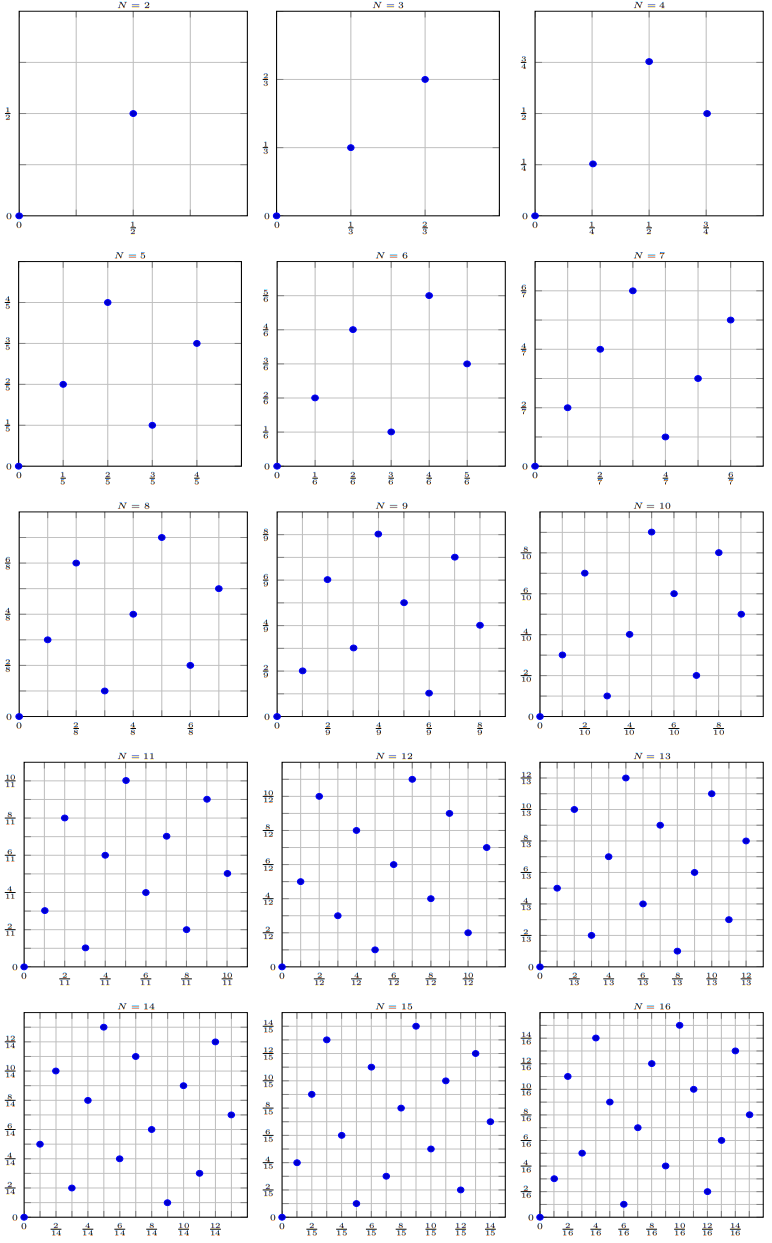
\includegraphics[width=160mm, height=250mm]{Figuras/Hinrichs.png}\par
    \caption{Optimal point sets for Quasi-Monte Carlo integration of bivariate periodic functions. Optimal point sets from $N=2$ to $N=16$ points and $\gamma = 1$ are shown (\cite{Hinrichs.pdf}). These are the points used for the Hinrichs method.}
    \label{fig:Hinrichs}
  \end{center}
\end{figure}








\end{document}



